%
% Template for Doctoral Theses at Uppsala 
% University. The template is based on    
% the layout and typography used for      
% dissertations in the Acta Universitatis 
% Upsaliensis series                      
% Ver 5.2 - 2012-08-08                  
% Latest version available at:            
%   http://ub.uu.se/thesistemplate            
%                                         
% Support: Wolmar Nyberg Akerstrom        
% Thesis Production           
% Uppsala University Library              
% avhandling@ub.uu.se                          
%                                         
%%%%%%%%%%%%%%%%%%%%%%%%%%%%%%%%%%%%%%%%%%%


\documentclass{UUThesisTemplate}

% Package to determine wether XeTeX is used
\usepackage{ifxetex}

\ifxetex
	% XeTeX specific packages and settings
	% Language, diacritics and hyphenation
	\usepackage[babelshorthands]{polyglossia}
	\setmainlanguage{english}

	% Font settings
	\setmainfont{Times New Roman}
	\setromanfont{Times New Roman}
	\setsansfont{Arial}
	\setmonofont{Courier New}
\else
	% Plain LaTeX specific packages and settings
	% Language, diacritics and hyphenationsudo apt install chktex
    % Use English and Swedish languages. 
	\usepackage[english]{babel} 

	% Font settings
	\usepackage{type1cm}
	\usepackage[latin1]{inputenc}
	\usepackage[T1]{fontenc}
	\usepackage{mathptmx}
	
	% Enable scaling of images on import
	\usepackage{graphicx}
\fi


% Tables
\usepackage{booktabs}
\usepackage{tabularx}

% Document links and bookmarks
\usepackage{hyperref} 

\usepackage{minted}

% Numbering of headings down to the subsection level
\numberingdepth{subsection}

% Including headings down to the subsection level in contents
\contentsdepth{subsection}


% Uncomment to use a custom abstract dummy text
\abstractdummy{
    \begin{abstract}
  Please use no more than 300 words and avoid mathematics or complex script.
\end{abstract}
}


\begin{document}
\frontmatter
% Creates the front matter (title page(s), abstract, list of papers)
% for either a Comprehensive Summary or a Monograph.
% Authors of Comprehensive Summaries use this front matter 
\frontmatterCS
% Monograph authors use this front matter 
%\frontmatterMonograph 

% Optional dedication
\dedication{Dedicated to all those whom tried and failed, who then tried and learnt}

\begingroup
% To adjust the indentation in your table of contents, uncomment and enter the widest numbers for each level
%  E.g.  \settocnumwidth{widest chapter number}{widest section number}{widest subsection number}...{...}
%  \settocnumwidth{5}{4}{5}{3}{3}{3}
\tableofcontents
\endgroup

% Optional lists
% \listoftables
% \listoffigures

\mainmatter
\part{Introduction}
\textit{If you can't measure it, you can't improve it -Peter Drucker}

\chapter{Background}
Containerization (or OS-Level Virtualization) \cite{virtualization} revolutionized the business world in 2013 with the introduction of Docker \cite{docker}.
Coupled with the high adoption rate of containerization saw the rapid adoption of container-orchestration tools (with the most popular being Kubernetes\cite{k8s}).

In parallel to the adoption of the aforementioned technologies, cloud-computing providers matured from offering basic compute, storage,
and networking offerings; to more managed "cloud-native" services.Amazon Web Services (AWS),
for example announced an early version of their custom container-orchestration tool (ECS) in 2015 \cite{ecs},
expanding their container-orchestration offerings with a serverless container platform (Fargate) in 2017\cite{fargate},
and a managed Kubernetes Engine (EKS) in 2018 \cite{eks}.
More recently, AWS has announced the ability to run containers as Lambdas (Serverless Functions) in late 2020\cite{lambda}.

\noindent These shifts in technological maturity enables workloads to fully leverage the advantages of containerization, with those offered by the cloud.
Unfortunately, the partition between the cloud offered container platforms are not entirely clear and rather fuzzy
(this includes performance, security, efficiency, latency and cost).\\

\noindent This Masters thesis project was conducted at Department of Information Technology at Uppsala University.
The project was undertaken in partnership with Allan Gray[\ref{sec:allan_gray}].

\section{Allan Gray}
\label{sec:allan_gray}
Allan Gray\cite{allan_gray} is a Africa's largest privately-owned and independent investment management company, with a primary focus on unit trusts.
Allan Gray hosts over 1200 employees, spread over four cities in South Africa. From these 1200, approximately 10\% are found within the I.T space,
and within the IT space at least 90\% are considered to be within a developer role.

\noindent Allan Gray is no exception to the aformentioned scenario. Allan Gray has been running container workloads in production for over five years,
running on the Kubernetes platform, on an on-premise data-center on virtual Linux machines.
Allan Gray is currently undertaking a cloud-migration, and is looking to shift their container-workloads to the cloud (with AWS being their chosen cloud platform).

\chapter{Goal}
\noindent The \textbf{goal} of this project is to investigate and compare cloud container orchestration platforms, in terms of:
\begin{itemize}
  \item ease of adoption and configuration
  \item deployment process
  \item restrictions and limitations
  \item performance
  \item cost impacts
  \item reliability and resilience
  \item security
\end{itemize}

\chapter{Delimitations}
This project is restricted to investigation and experimentation pertaining to:
\begin{itemize}
  \item container-based workloads
  \item the Amazon Web Services Cloud provider
\end{itemize}

\section{Justifying the choice of focusing solely on AWS}
Whilst it seems that experimenting only on AWS severely restricts the generality of this investigation, in reality the offerings by the other two major cloud providers
(being Google Cloud Platform and Microsoft Azure Cloud respectively), match the Cloud Orchestrated Container offerings by AWS at a feature-parity level \cite{contaier_workloads}.
Additionally, AWS holds more that 33\% of the cloud market (as of Q4 2021) \cite{aws_cloud_share},
and is considered to be the cloud-provider of choice for the the largest tech companies in the world today \cite{aws_users}.

Therefore the broader results of this investigation (and recommendations) would (in theory) apply to the GCP and Azure cloud as well.

\chapter{Structure}
% This thesis is structured as follows: Section 2 covers the background and
% related work. Section 3 introduces methods used in the development, design
% of the system and the evaluation method in detail. In Section 4, we describe
% and discuss the results and the evaluation results. In section 5, we conclude
% results, limitations of the thesis and describe the future work
% \noindent A \textit{quantitative} analysis will be presented, using the results from the experimentation phase.
% However a \textit{qualitative} analysis will also be presented, with data gathered via interviews of developers, to better understand their requirements of a solution.

\part{Theory, Terminology, and Related Work}
\label{sec:theory}

Before analyzing the problem or providing a solution,
this chapter defines briefly the technologies and terminology used in this project.
Additionally an overview of related work is presented.

\chapter{Cloud Computing}
First coined in 1997\cite{ray2018} in an address to the INFORMS Annual meet, 
Chellapa \cite{chellappa1997intermediaries} defined Cloud Computing as a
\emph{computing paradigm where the boundaries of computing will be determined by economic rationale rather than technical limits alone}. 

Haris and Kahn\cite{haris2018systematic} provide a more expanded definition as \emph{an advancement of various combined technologies such as 
Distributed computing, Utility computing, virtualization etc, to provide IT resources and services over an internet on pay as per use manner. 
These services are available to the user on demand basis at very low cost and charged at the time of the release of resources. 
These services include storage, processing, network, application, etc}. 

\section{Cloud Computing technologies used in this project}

\subsection{Virtual Private Cloud (VPC)}
AWS defines a VPC as a virtual network which closely resembles a traditional network that would be operated in an \emph{on-premise} data center, 
with the benefits of using the scalable infrastructure of AWS, wherein cloud resources can be launched.\cite{awsdocs_2022}
Beach et al. further explain that a \emph{VPC allows you to configure a custom network topology, as well as manage IP routing and security. 
A network topology is the structure of the network and controls how data flows between nodes.}\cite{Beach2019}

\subsection{Regions \& Availability Zones (AZ)}
Carty defines regions as \emph{geographic locations in which public cloud service providers' data centers reside} 
and Availability Zones as \emph{isolated locations within data center regions from which public cloud services originate and operate}.\cite{carty_2015}

That is to say a public cloud service provider could have multiple isolated data-centers (zones) within a specific geographical region of operation.
Cloud resources can be deployed to various regions (and by extension specific zones) for redundancy and availability.

\subsection{Elastic Compute Cloud (EC2)}
Amazon Elastic Compute Cloud (Amazon EC2) provides scalable computing capacity in the Amazon Web Services (AWS) Cloud\cite{awsdocs_whatsisec2}.
It achieves this by allowing the creation of on-demand \emph{Virtual Machines} in the cloud called \emph{instances}\cite{carty_2019}. 
These instances can be of varying specifications \cite{daly_2022} and run various operating systems \cite{awsdocs_ec2os} per requirement.

\subsubsection{Amazon Machine Image (AMI)}
An Amazon Machine Image (AMI) is a template that contains a software configuration (for example, an operating system, an application server, and applications)\cite{awsdocs_ami}.
AMIs are published by AWS, software vendors, or can be created by users themselves to contain specific application software or configuration required per instance.
These templates are used to create EC2 instances\cite{Beach2014}. 

\subsubsection{Auto-Scaling Groups (ASG)}
AWS defines an ASG as a logical resource which \emph{contains a collection of Amazon EC2 instances that are treated as a logical grouping for the purposes of automatic scaling and management} \cite{awsdocs_asg}.
ASGs helps you ensure that you have the correct number of Amazon EC2 instances available to handle the load for your application by scaling up or down the number of active instances based on requirement \cite{amazon_asg_docs}. 
ASGs perform periodic health-checks on the instances within the group, replacing unhealthy instances with new instances to maintain availability.

\subsection{Security Groups (SG)}
AWS defines an SG as a logical resource which \emph{controls the traffic that is allowed to reach and leave the resources that it is associated with} \cite{amazon_2016}.
In essence it is a per instance set of \emph{stateful} rules which defines the allowed ingress and egress network activity per instance. 

\subsection{Relation Database Service (RDS)}
Lutkevich \cite{lutkevich_2021} defines RDS as \emph{a managed SQL database service provided by Amazon Web Services (AWS). Amazon RDS supports an array of database engines to store and organize data. 
It also helps with relational database management tasks, such as data migration, backup, recovery and patching.}

RDS supports MySQL, MariaDB, PostgreSQL, Oracle, and SQL Server \cite{beach2019relational}.

\chapter{Virtual Machines}
Defined by Popek and Goldburg in 1974 as \emph{an efficient, isolated duplicate of a real computer machine}\cite{popek_1974}. 
A VM is resource which uses software (by emulating physical hardware) to run operating systems, programs, and applications. 
Multiple isolated VMs can run as \textit{guests} on a single physical \textit{host} system, with each \textit{guest} VM reserving a portion of the underlying
\textit{host}'s hardware. 

VMs benefit from allowing easy restore points via \textit{snapshotting} (the ability to \textit{save} the entire state of a machine at any given point in time), 
and the ability to quickly create multiple VMs which share the same properties, configuration, and applications via \textit{cloning}\cite{n-able_2021}. 

Virtual Machines do have notable restrictions: infections from a \textit{host} system may spread to all \textit{guest} VMs;
the sharing and reservation of underlying hardware results in a \textit{host} system which may not be fully utilized, 
while leading to unpredictable performance for \textit{guest} VMs if the \textit{host} is under load. 
Finally due to the overhead of virtualization, the \textit{guest} VM generally performs slower than non-virtualized environments\cite{Martinovic}.

\chapter{Containerization}

Containerization (or OS-Level Virtualization \cite{10.5555/1571423}) is defined by Dua et al. as 
\emph{a light weight operating system running inside the host system, running instructions native to the core
CPU, eliminating the need for instruction level emulation or just in time compilation}\cite{6903537}.

Containers achieve the same benefits of VMs (including isolation) without the overhead of virtualization, therefore maintaining portability 
without the significant drop in performance seen by VMs \cite{POTDAR20201419}.

A more thorougher comparison between containers and VMs is presented in \cite[Table 1]{6903537}.

\section{Docker}
Docker \cite{docker} is an open-source container virtualization tool. 
It defines a standard for the building of container images (via text templates called \textit{Dockerfiles} which describe a container and its dependencies),
the distribution of container-images, and the creation and running of containers\cite{7093032}.

Rad et al. \cite{rad2017introduction} provide a deep analysis of Docker, including a break-down of the Docker architecture presented in \cite[Fig. 1]{rad2017introduction}

\section{Kubernetes (k8s)}
Kubernetes \cite{kubernetes} is an open-source tool for managing containerized services. 
Originally created by Google as Borg \cite{10.1145/2741948.2741964} abd being open-sourced in 2014\cite{metz_2014}. 

Docker is sufficient as a tool to run container-workloads locally or on single-system architectures when running low number of containers.
However, to fully leverage the power of containers, especially when running high number of containers across multiple host systems, additional features are required.
k8s provides a user with (in relation to container-workloads): service discovery and load-balancing; storage-orchestration; self-healing; automatic bin-packing; automated roll-outs and rollbacks; 
and secret and configuration management \cite{kubernetes_2022}.

Luksa \cite{luksa2017kubernetes} presents a deep-dive exploration of the k8s architecture and design, including the basic building blocks as illustrated by \cite[Figure 1.9]{luksa2017kubernetes}.


\section{AWS Elastic Container Service}
ECS is a custom cloud-native fully-managed container-orchestration service launched by AWS in 2014 \cite{ecs}.
ECS relies on the creation of an underlying cluster upon which container workloads are run.
ECS wraps container-workloads in an abstraction called a \textit{task}, which houses additional information required by the orchestration tool.
ECS ties in natively to other cloud-services (which include identity management, service discovery and load-balancing).
ECS can schedule tasks on both VM and Serverless platforms \cite{ecs_2022}.

\section{AWS Elastic Kubernetes Service}
EKS is a cloud fully-managed Kubernetes service launched by AWS in 2018 \cite{eks}. 
EKS obfuscates the control-plane portion of the k8s cluster, thus only exposing the worker-nodes to users.
EKS ties into cloud-native services via adaptors and therefore expands upon the standard kubernetes functionality.
EKS can also schedule tasks on both VM worker-nodes or Serverless workers\cite{hansen_2022}. 

\chapter{Serverless Computing}
\section{Serverless Functions}
\subsection{AWS Lambda Functions}
\section{Serverless Containers}
\subsection{AWS Fargate}

\chapter{Infrastructure as Code (IaC)}
Rahman et al. define IaC as \emph{the practice to automatically configure system dependencies and to provision local and remote instances}\cite{RAHMAN201965}.
IaC allows you to build, change, and manage your infrastructure in a safe, consistent, and repeatable way by defining resource configurations that you can version, reuse, and share\cite{hashicorp_tf_iac}.

IaC allows for easy deployment of identical resources to multiple environments, 
can follow standard code review processes, and can make use of a source-control system (like git).

Common IaC tools include: chef\cite{chef}, puppet\cite{puppet}, ansible\cite{ansible}, Terraform\cite{terraform}, and packer\cite{packer}. 
This project will be utilizing Terraform and packer.
 
\section{Terraform (tf)}
Terraform created by HashiCorp\cite{hashicorp}, is an open-source IaC software tool. 
tf scripts are written in HashiCorp Configuration Language (HCL) or JSON, and can target both cloud and on-premise resources.
tf utilizes \textit{providers} to communicate with services via their APIs, therefore tf is extendible to any service with public APIs. 

Terraform uses a declarative configuration model to describe a desired final state. Upon deployment, tf first checks the current state of the service,
and compares it to the saved state (that is the state at the end of the last deployment). Any external changes are noted and reverted to that which is declared in code.
Finally tf attempts to change the current state of the service to the desired state declared by the user by making the required API calls.

\section{packer}
Terraform created by HashiCorp\cite{hashicorp}, is an open-source machine image IaC build and creation tool. 
Generally used to create \emph{golden-images} \cite{HashiCorp_packer_docs} (that is base-level machine image which contains all requirements and configuration for a given provider).

packer (similarly to Terraform) makes use of public APIs to create and configure machine images with various \textit{builders}, and benefits from the same advantages which IaC tooling provides.


\chapter{Other Terms and Concepts}
\section*{Rancher Kubernetes Engine (RKE)}
RKE is a Kubernetes distribution which runs entirely using Docker containers \cite{rke}. 

\section*{LZMA}
LZMA compression is a type of data-compression algorithm.
It was designed by Igor Pavlov as part of the 7zip \cite{pavlov_2022} project and was first implemented in 1998.
The name \textit{LZMA} stands for \textit{Lempel-Ziv Markov chain Algorithm}\cite{winzip_2021}

\section*{CRUD}
In computer programming, Create, Read, Update, and Delete are the four basic operations of persistent storage\cite{martin1983managing}.

\section*{Orchestration}
Orchestration is the automated configuration, coordination, and management of computer systems and software\cite{erl1900service}.

\section*{Chaos-Engineering}
Chaos Engineering is the discipline of experimenting on a system in order to build confidence in the system's capability to withstand turbulent conditions in production\cite{hochstein_2019}.

\section*{Time-to-recover (TTR)}
The measure of time between a service being down, until service is restored.

\section*{Service Level Agreements (SLAs)}
Service Level Agreements (SLAs) are a common way to formally specify the exact
conditions (both functional and non-functional) under which services are or should
be delivered \cite{wieder2011service}.


\chapter{Related Work}

\part{Methodology and System Architecture}
\chapter{Experimentation Methodology}

\chapter{System Design and Architecture}
\section{Environment}
\chapter{Results}
\label{sec:results}

This chapter presents the relevant results of the investigation and experimentation phases.
Presenting the tested cloud container orchestration platforms first,
followed by the results per evaluation requirement thereafter.

\section{Viable Solutions}
The following platforms were evaluated as potential solutions:
\begin{itemize}
  \item AWS Lambda (representing \textit{Serverless Functions})
  \item AWS ECS (representing \textit{Cloud Native})
        \begin{itemize}
          \item running on EC2 (representing \textit{Virtual Machines})
          \item running on Fargate (representing \textit{Serverless Containers})
        \end{itemize}
  \item AWS EKS (representing \textit{Kubernetes})
        \begin{itemize}
          \item running on EC2 (representing \textit{Virtual Machines})
          \item running on Fargate (representing \textit{Serverless Containers})
        \end{itemize}
\end{itemize}

\section{Experimentation Results}

\subsection{Performance and Latency}
Each platform was subjected to an identical set of broad benchmarks aiming to fully test the impact of both
selection of \emph{orchestration platform} and \emph{underlying architecture} in relation to performance.

\subsubsection{CPU}
\begin{figure}[htbp]
  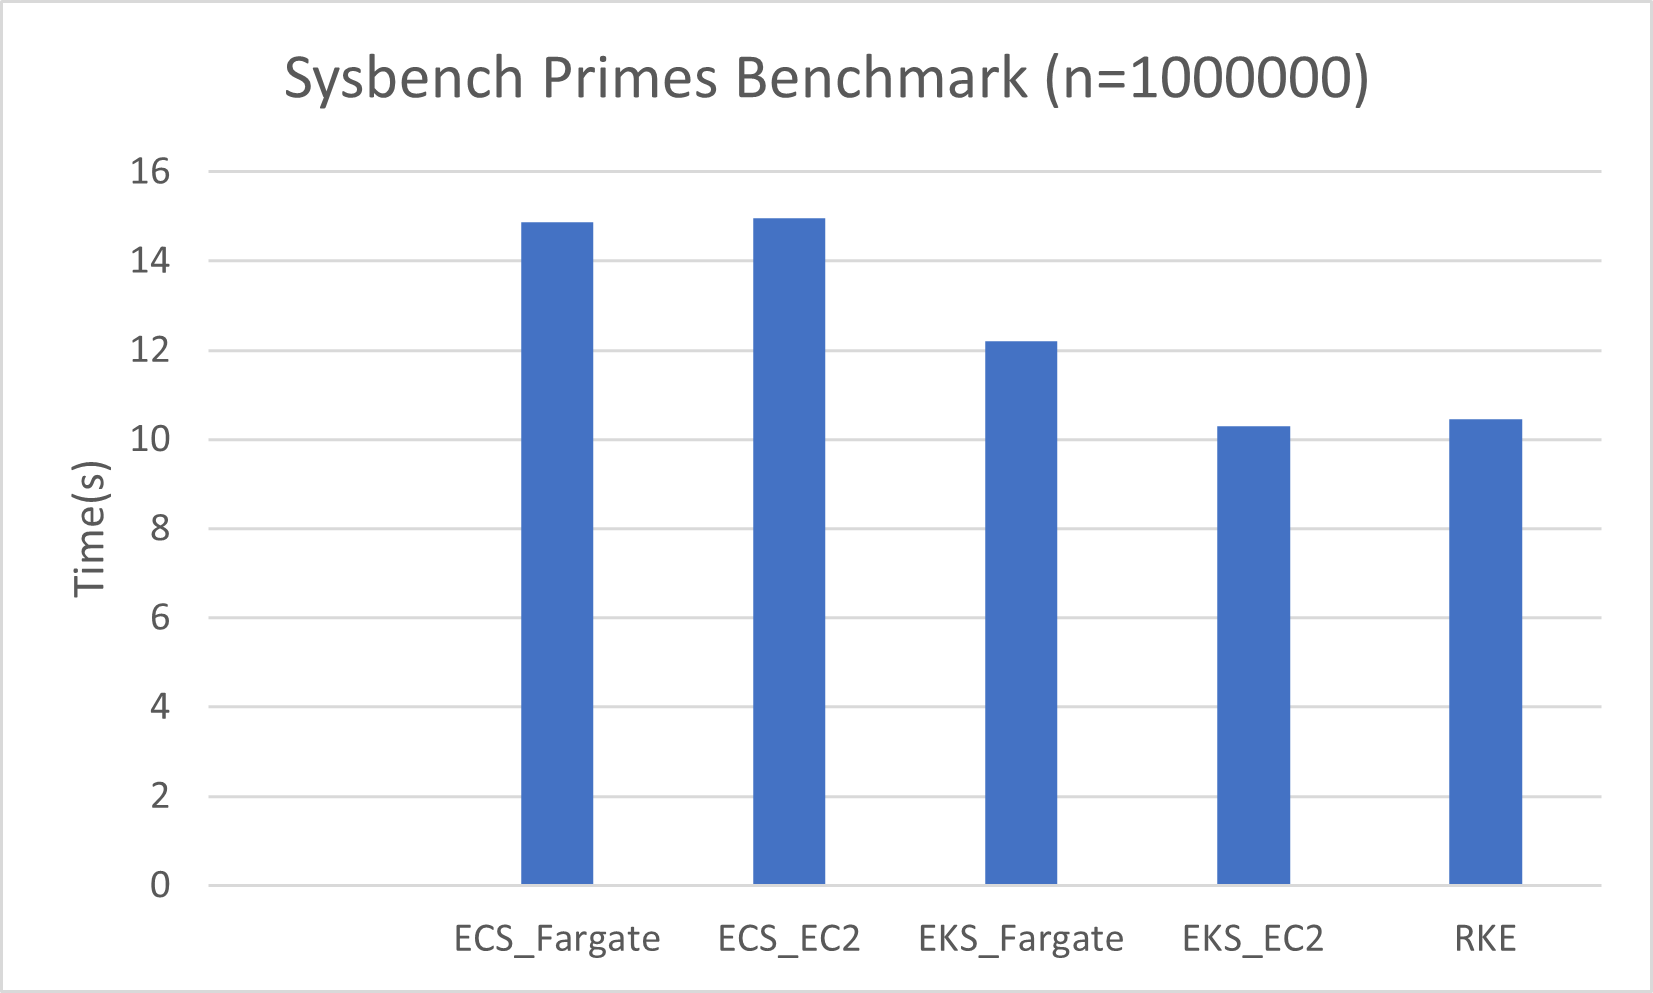
\includegraphics[width=\textwidth]{images/perf-sysbench.png}
  \caption{\emph{Performance}: Average time taken to compute primes up to 1000000 --- lower is better }
  \label{fig:perf_sysbench}
\end{figure}

\begin{figure}[htbp]
  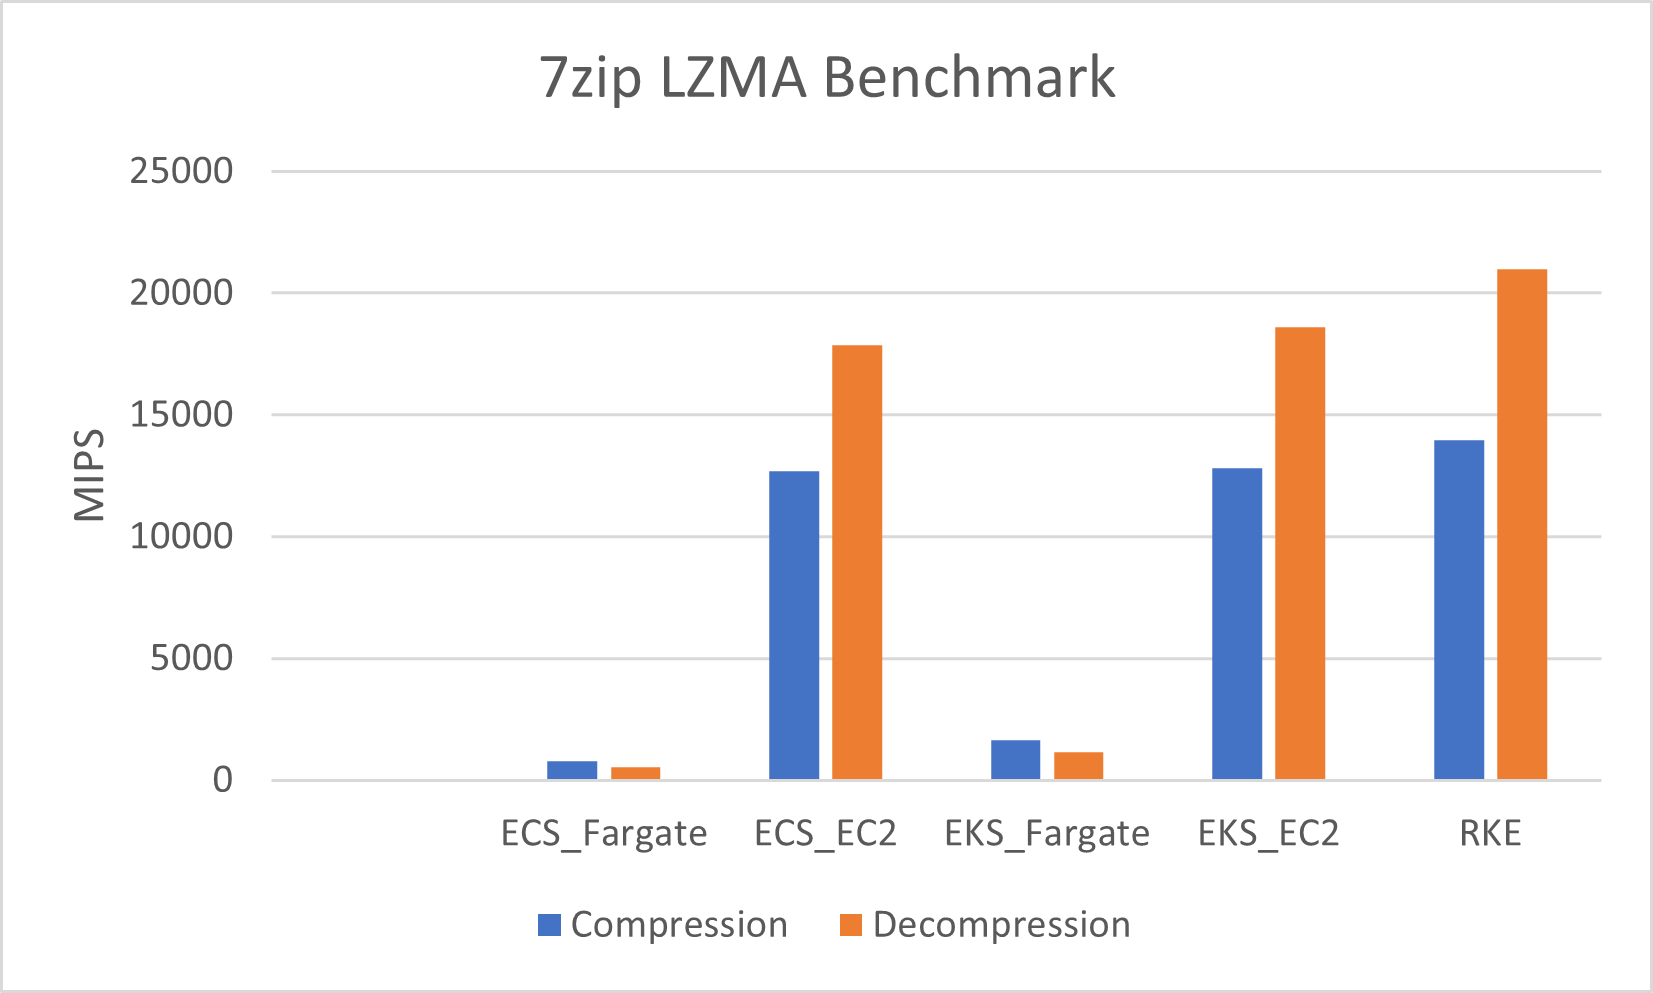
\includegraphics[width=\textwidth]{images/perf-7zip.png}
  \caption{\emph{Performance}: Average rating in MIPS to complete the 7zip LZMA Benchmark --- higher is better}
  \label{fig:perf_7zip}
\end{figure}

CPU performance was evaluated by performing CPU intensive tasks, such as computing prime numbers using a prime sieve,
and archive compression/ decompression and measuring the time taken to complete the respective tasks.

Figure \ref{fig:perf_sysbench} illustrates the amount of time taken (s) to compute primes up to 1000000 across 4 threads using \textit{Sysbench}.
The \textit{EC2} instance of the \textit{EKS} cluster outperformed the baseline \textit{RKE} instance by a margin of ~2\%,
with the \textit{fargate} solution performing 20 \% slower than the baseline.
Finally, both the \textit{ECS} backed instances completed the task about 50\% slower than the baseline. 

Figure \ref{fig:perf_7zip} illustrates the rating in million of instructions per second (MIPS) when performing the 7zip \textit{LZMA} compression and decompression benchmark.
Under this benchmark, the baseline \textit{RKE} instance posted the best result, with the two \textit{EC2} backed instances completing around 9\% (\textit{EKS}) and 10 \% (\textit{ECS}) less instructions respectively.
The two \textit{fargate} backed instances struggled immensely to complete this benchmark,
with the \textit{EKS} instance completing 80\% less tasks, and the \textit{ECS} instance completing 95 \% less tasks.

\noindent \newline It should be noted that due to runtime, and execution time-limit, limitations \textit{Lambda} did not complete in these CPU specific benchmarks.

\subsubsection{Memory}
Two criterion of memory performance was evaluated, the first being \emph{speed},
which was evaluated using the RAMSpeed, and \emph{bandwidth} using the MBW tool.

RAMSpeed performs four distinct memory intensive tasks with results, each measuring a different aspect of memory performance.
All results are recorded as a measurement of speed (MB/S).

This discussion will focus on last column in Figure \ref{fig:perf_RAMSpeed} as it illustrates the average speed recorded for the entirety of the benchmark (that is all four distinct tasks),
as the results (and performance difference) found in this table is wholly illustrative to the results found in each of the sub-tasks.
The \textit{EC2} backed \textit{EKS} instance outperformed the baseline \textit{RKE} instance by completing the tasks close to 36\% quicker.
This was followed by a significantly slower \textit{fargate} backed instance of \textit{EKS}, and \textit{EC2} backed \textit{ECS} instance,
which both completed close to 80\% slower than the baseline.
Finally the \textit{fargate} backed \textit{ECS} instance completed the benchmark close to 88\% slower.

\begin{figure}[htbp]
  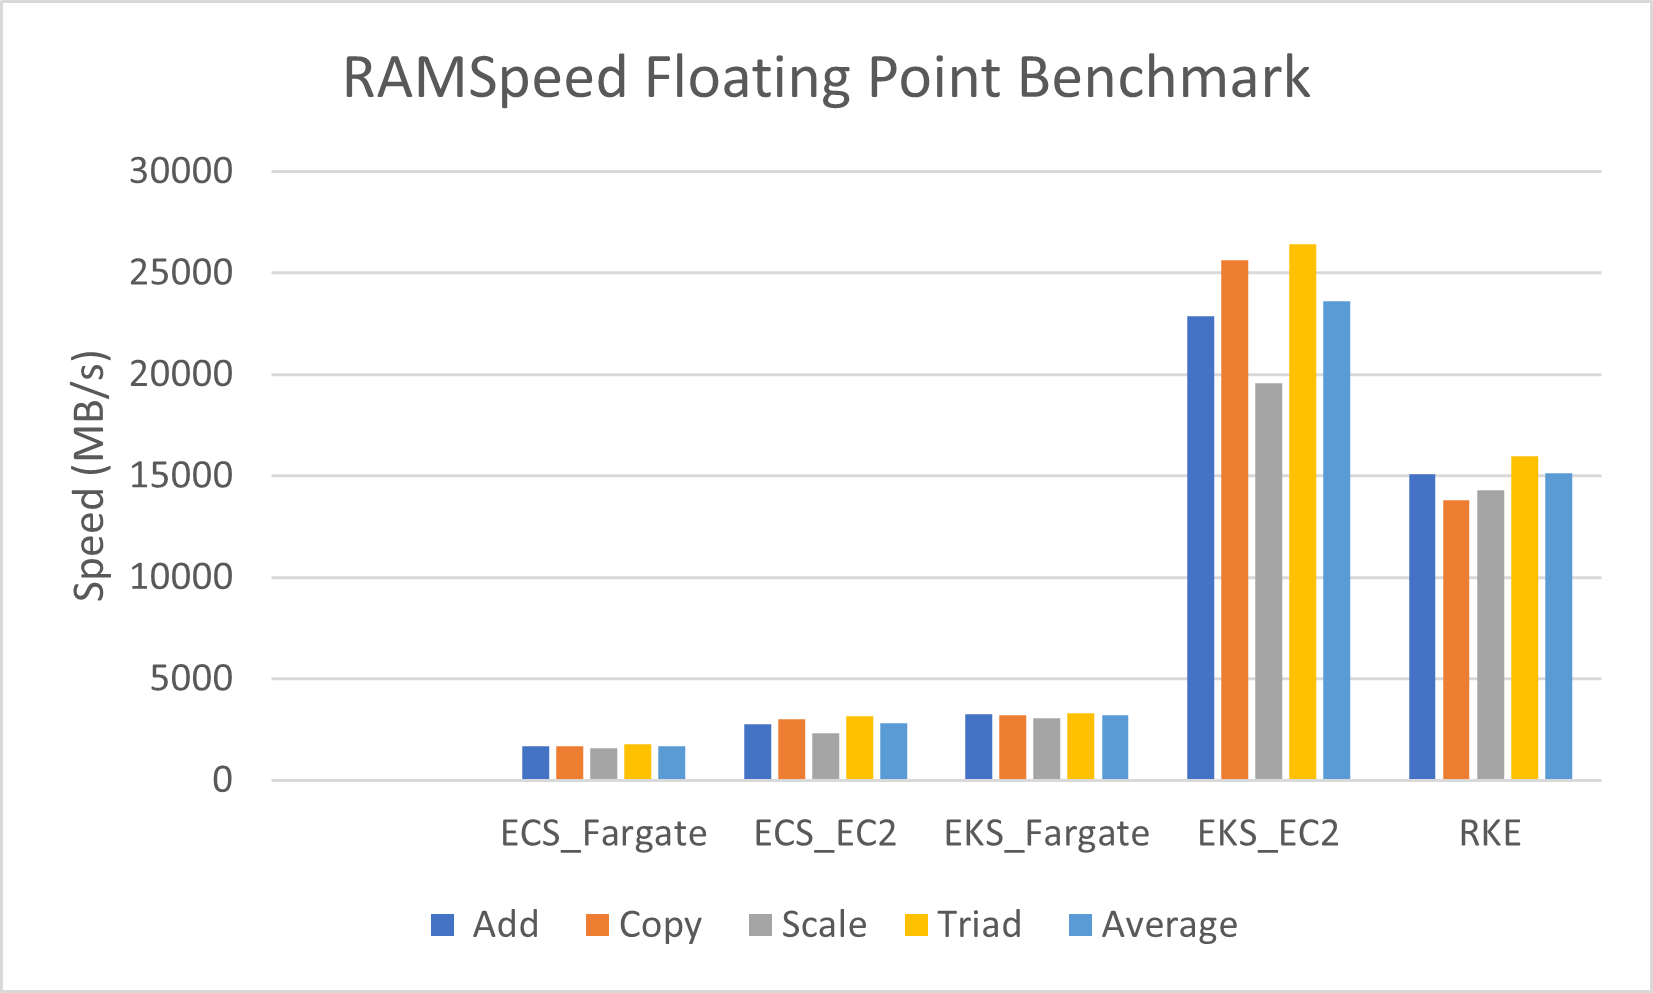
\includegraphics[width=\textwidth]{images/perf-RAMSpeed.png}
  \caption{\emph{Performance}: Average maximum speed achieved whilst completing the RAMSpeed Benchmark --- higher is better}
  \label{fig:perf_RAMSpeed}
\end{figure}

\begin{figure}[htbp]
  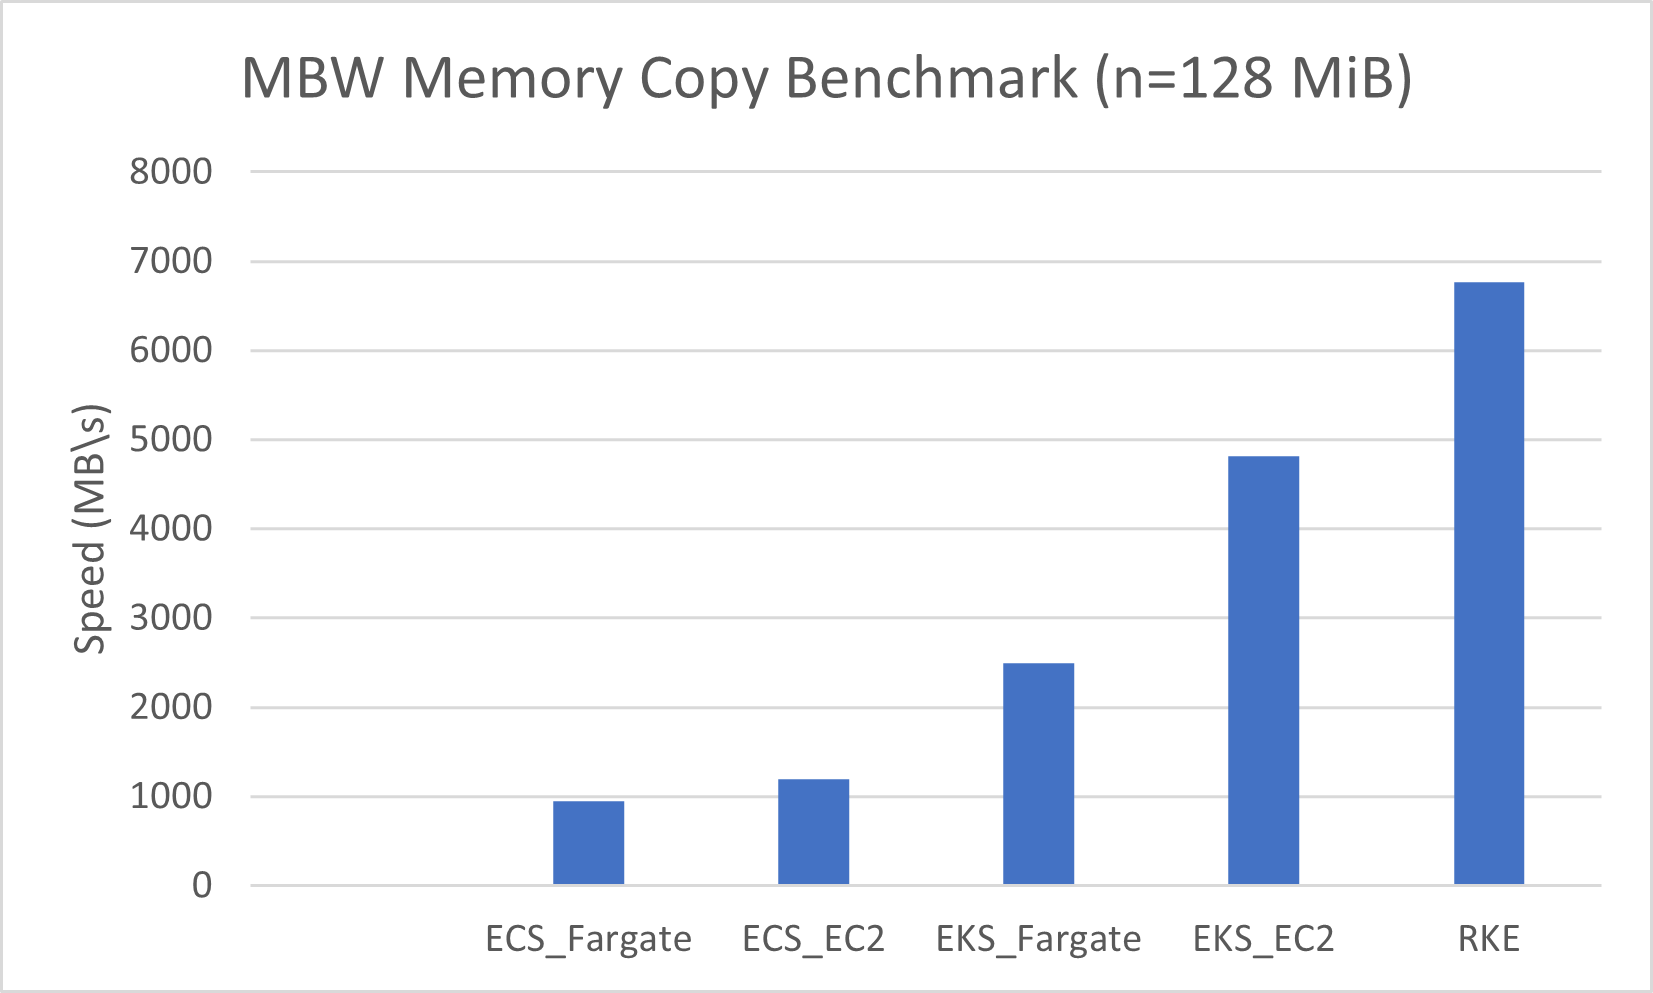
\includegraphics[width=\textwidth]{images/perf-MBW.png}
  \caption{\emph{Performance}: Average maximum speed achieved whilst completing the Memory Bandwidth Benchmark --- higher is better}
  \label{fig:perf_MBW}
\end{figure}

\noindent \newline MBW measures the amount of copy memory bandwidth available to a user-application in terms of speed (MB/s).

Figure \ref{fig:perf_MBW} illustrates the baseline \textit{RKE} instance completed this benchmark with the fastest speed, with the \textit{EC2} backed \textit{EKS} instance following at 29\% slower.
The \textit{fargate} backed \textit{EKS} instance completed 64\% slower,
followed by the two \textit{ECS} workloads at 83\% and 87\% slower for the \textit{EC2} and \textit{fargate} instances respectively.

\noindent \newline It should be noted that due to runtime, and execution time-limit, limitations \textit{Lambda} did not complete in these Memory specific benchmarks.

\subsubsection{I/O}
fs\_mark evaluates a system's underlying file-system by performing heavily synchronous IO tasks across multiple folders/drives, measured in terms of speed (number of files per second).

Figure \ref{fig:perf_FSMark} illustrates the \textit{EC2} backed \textit{ECS} instance outperforming the baseline \textit{RKE} instance by close to 64\%,
followed closely by the \textit{EC2} backed \textit{EKS} instance which outperformed the baseline by close to 63\%.

\begin{figure}[htbp]
  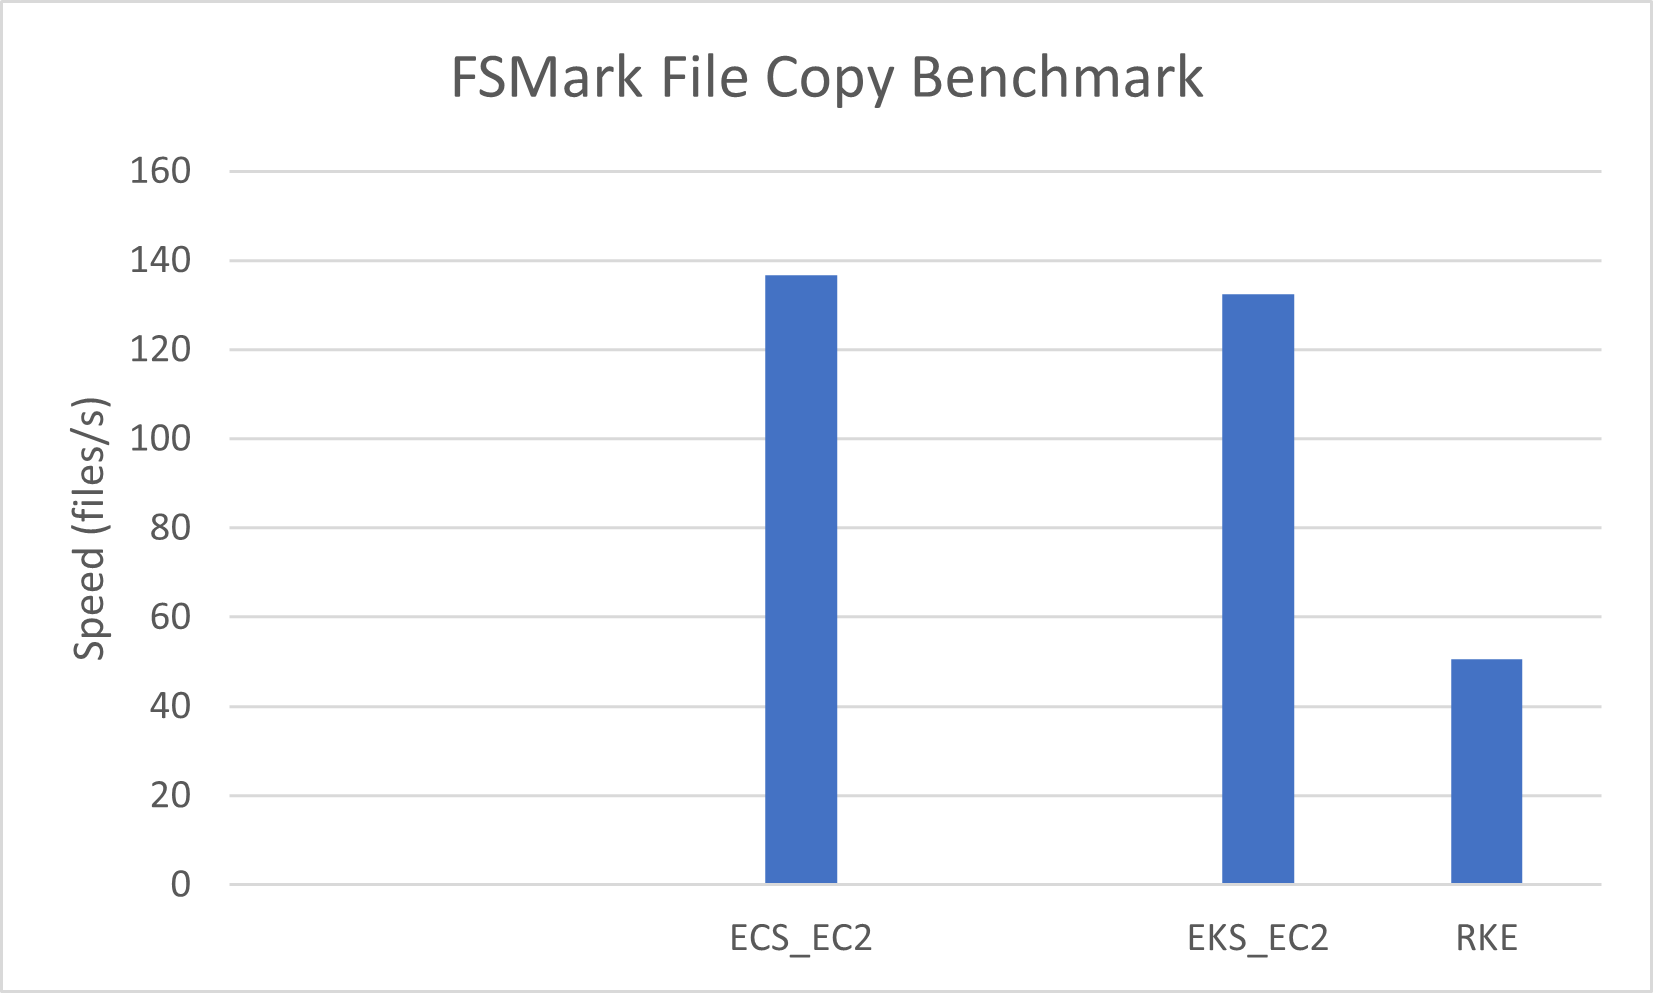
\includegraphics[width=\textwidth]{images/perf-FSMark.png}
  \caption{\emph{Performance}: Average maximum speed achieved whilst completing the fs\_mark Benchmark --- higher is better}
  \label{fig:perf_FSMark}
\end{figure}

\noindent \newline It should be noted that due to file-system mount limitations, neither of the \textit{Serverless} backed instances (that is \textit{Lambda} and \textit{fargate}) were able to complete these I\/O specific benchmarks.

\subsubsection{General Workloads}
In addition to focused hardware specific benchmarks (which are not often illustrative of real-world performance),
the following benchmarks were run to simulate performance under daily-tasks.

\paragraph{m-queens}
m-queens solves the \emph{n-queens} problem using multi-threading, measured in terms of time-to-completion (s).

Figure \ref{fig:perf_mQueens} shows the baseline \textit{RKE} cluster complete in the quickest amount of time,
followed by the \textit{EC2} backed \textit{EKS} instance almost 50\% slower.
The other instances completed this task an order of magnitude slower, all completing close to 99\% slower than baseline.

\begin{figure}[htbp]
  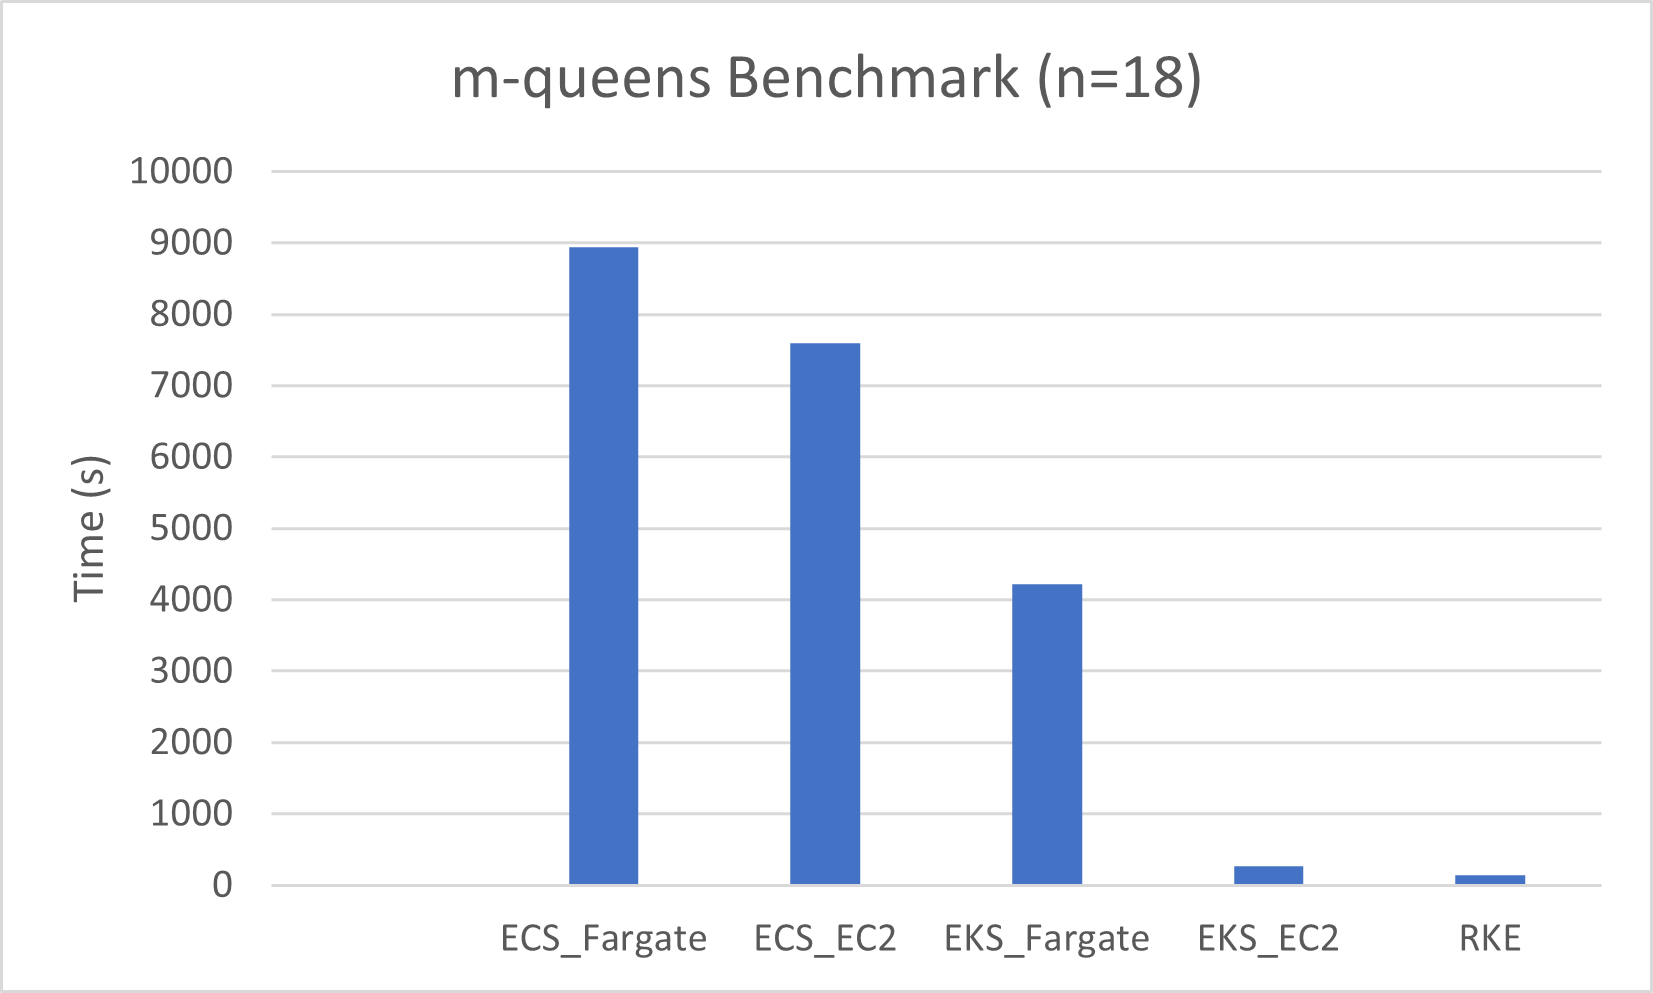
\includegraphics[width=\textwidth]{images/perf-m_queens.png}
  \caption{\emph{Performance}: Average amount of time required to solve the n-queens problem (n=18) --- lower is better}
  \label{fig:perf_mQueens}
\end{figure}

\paragraph{tool-container-benchmark}
\emph{tool-container-benchmark} simulates a general \textit{CRUD} based workload at load, measured in terms of time-to-completion (m).

Due to extreme network latency in terms of the database, the set of benchmarks were run twice,
first against an on-premise database, and the second against a cloud-hosted \textit{RDS} instance (illustrated by Figure \ref{fig:perf_tcb_default}).
Additionally in an attempt to cater for \textit{Lambda}, the set of benchmarks were re-run with a limit of 30000 \emph{events},
against both the on-premise and RDS databases
(illustrated by Figure \ref{fig:perf_tcb_30000}).

The \textit{RDS} series in Figure \ref{fig:perf_tcb_default} illustrates the \textit{EC2} backed \textit{EKS} instance performing the quickest,
followed by the two \textit{ECS} instances, with the \textit{fargate} backed and \textit{EC2} instances completing 9\% and 14\% slower respectively.
Finally, the \textit{fargate} backed \textit{EKS} instance completed the slowest (excluding the baseline \textit{RKE} instance).

The \textit{RDS} series in Figure \ref{fig:perf_tcb_30000} illustrates an anomaly with the \textit{fargate} backed \textit{ECS}
instance completing around 40\% quicker than the other instances, with all other instances completing within 30s of each other
except for \textit{Lambda} which completed close to 64\% slower.

\begin{figure}[htbp]
  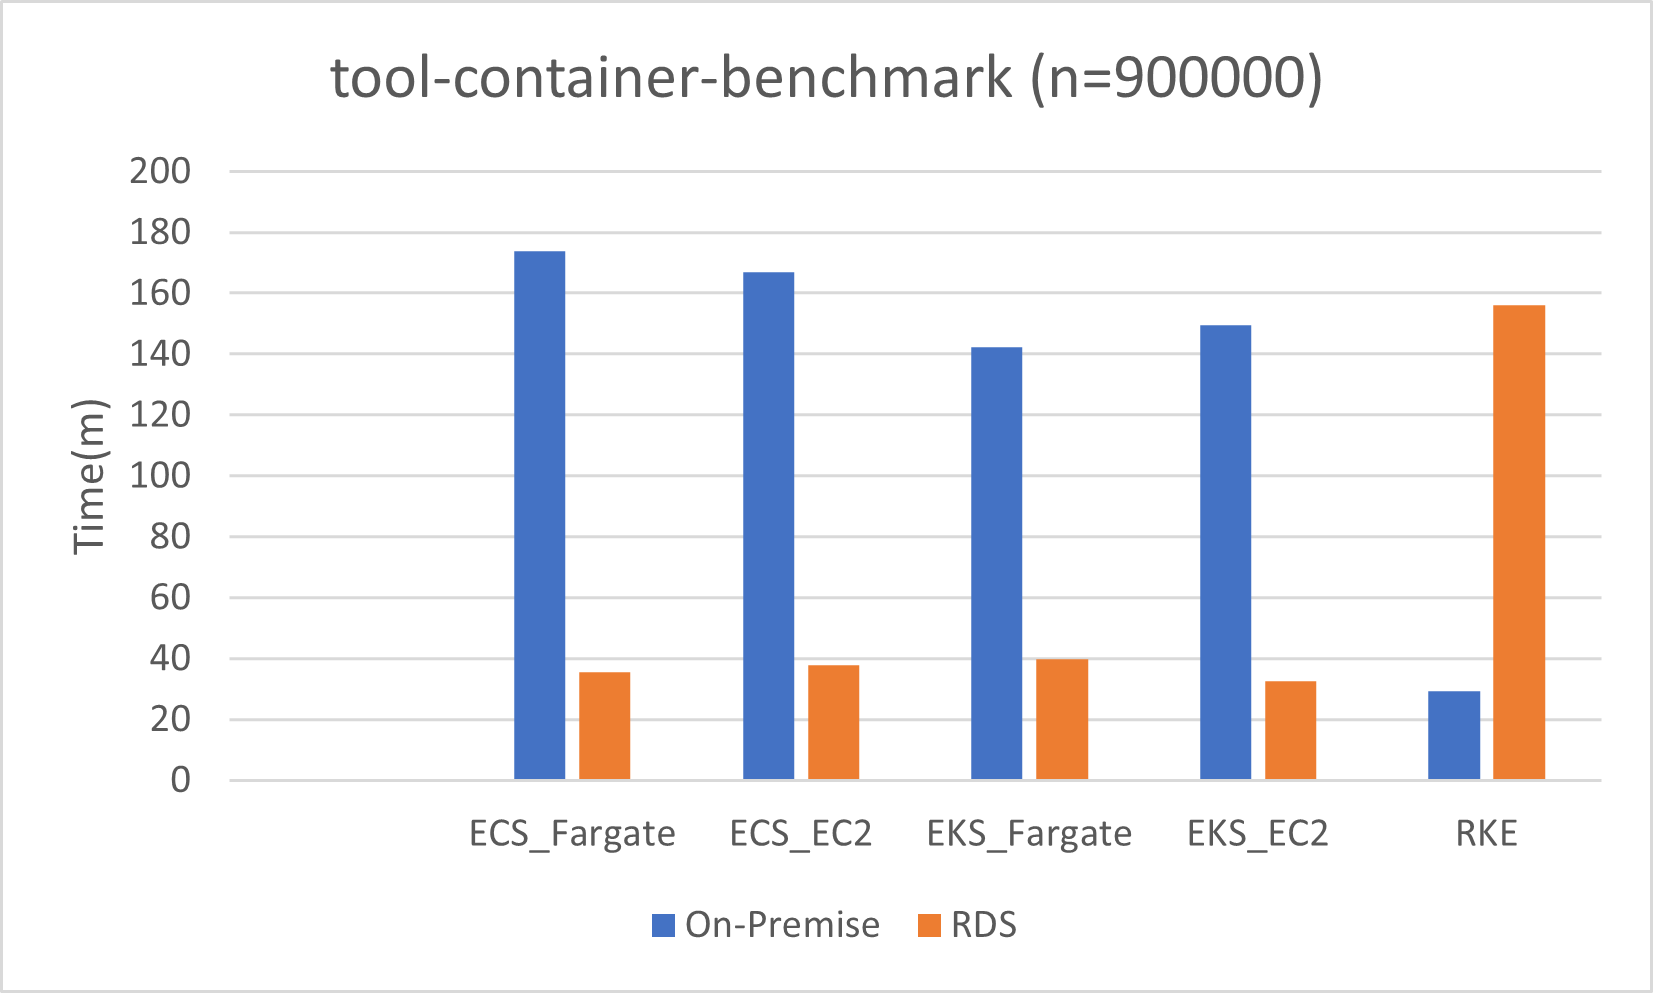
\includegraphics[width=\textwidth]{images/perf-tcb_default.png}
  \caption{\emph{Performance}: Average amount of time required to complete tool-container-benchmark (number\_of\_events=9000000) --- lower is better}
  \label{fig:perf_tcb_default}
\end{figure}

\begin{figure}[htbp]
  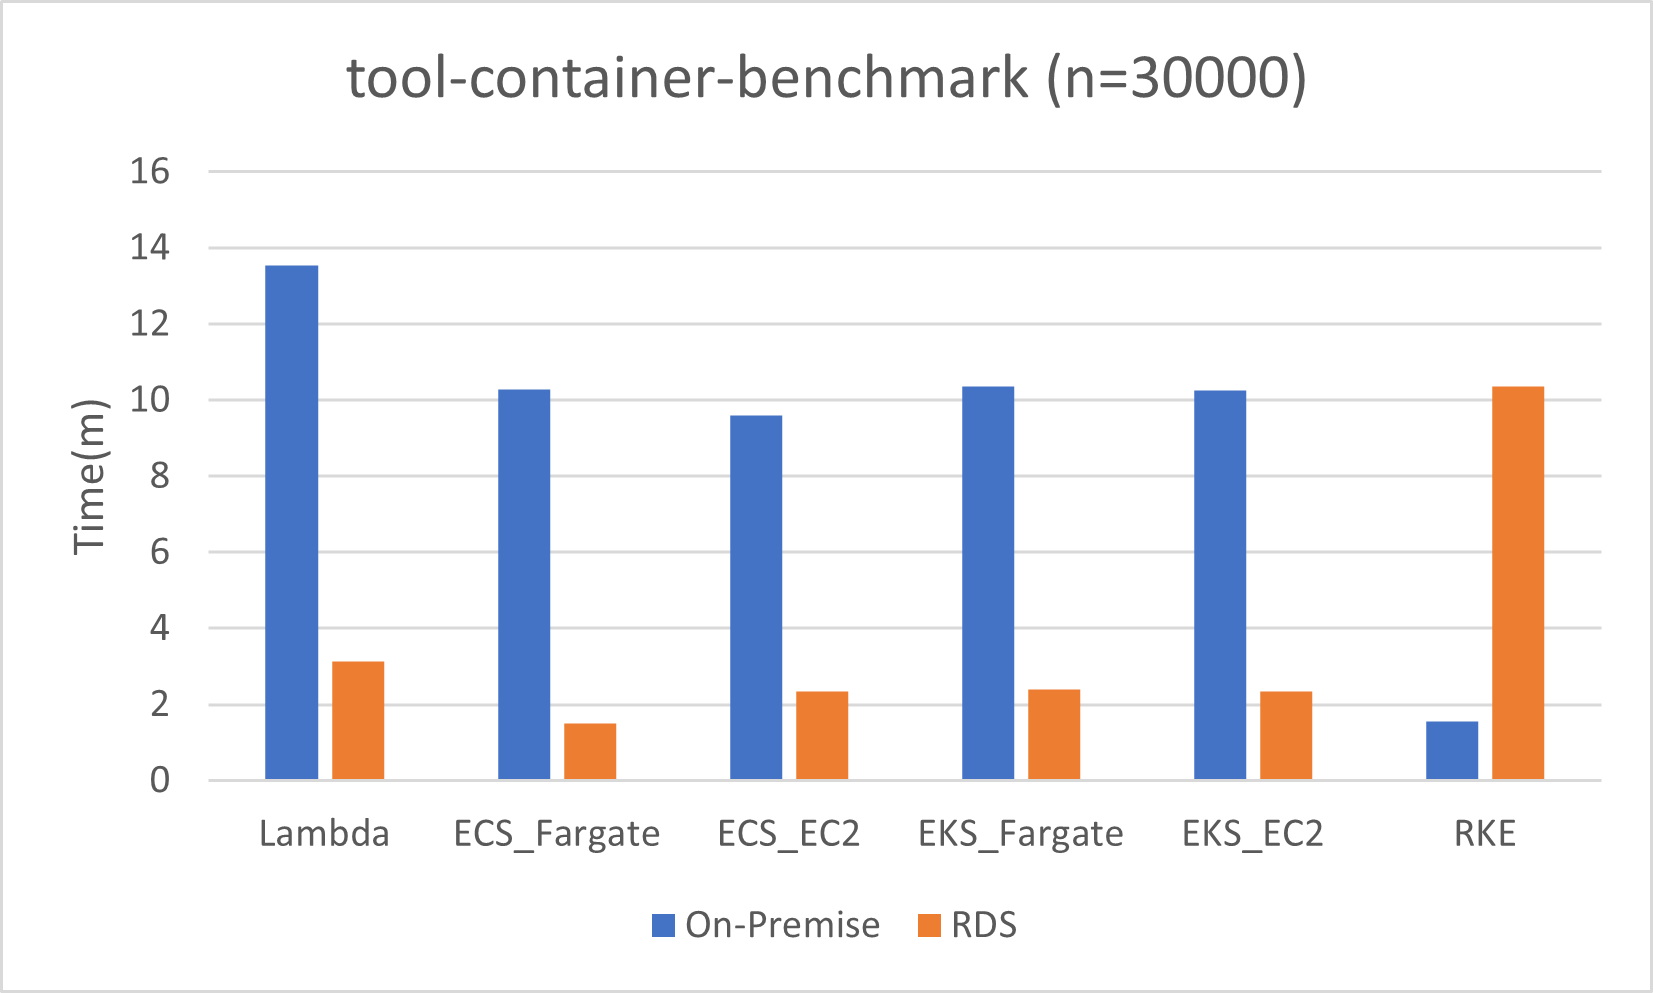
\includegraphics[width=\textwidth]{images/perf-tcb_30000.png}
  \caption{\emph{Performance}:Average amount of time required to complete tool-container-benchmark (number\_of\_events=30000) --- lower is better}
  \label{fig:perf_tcb_30000}
\end{figure}

\begin{figure}[htbp]
  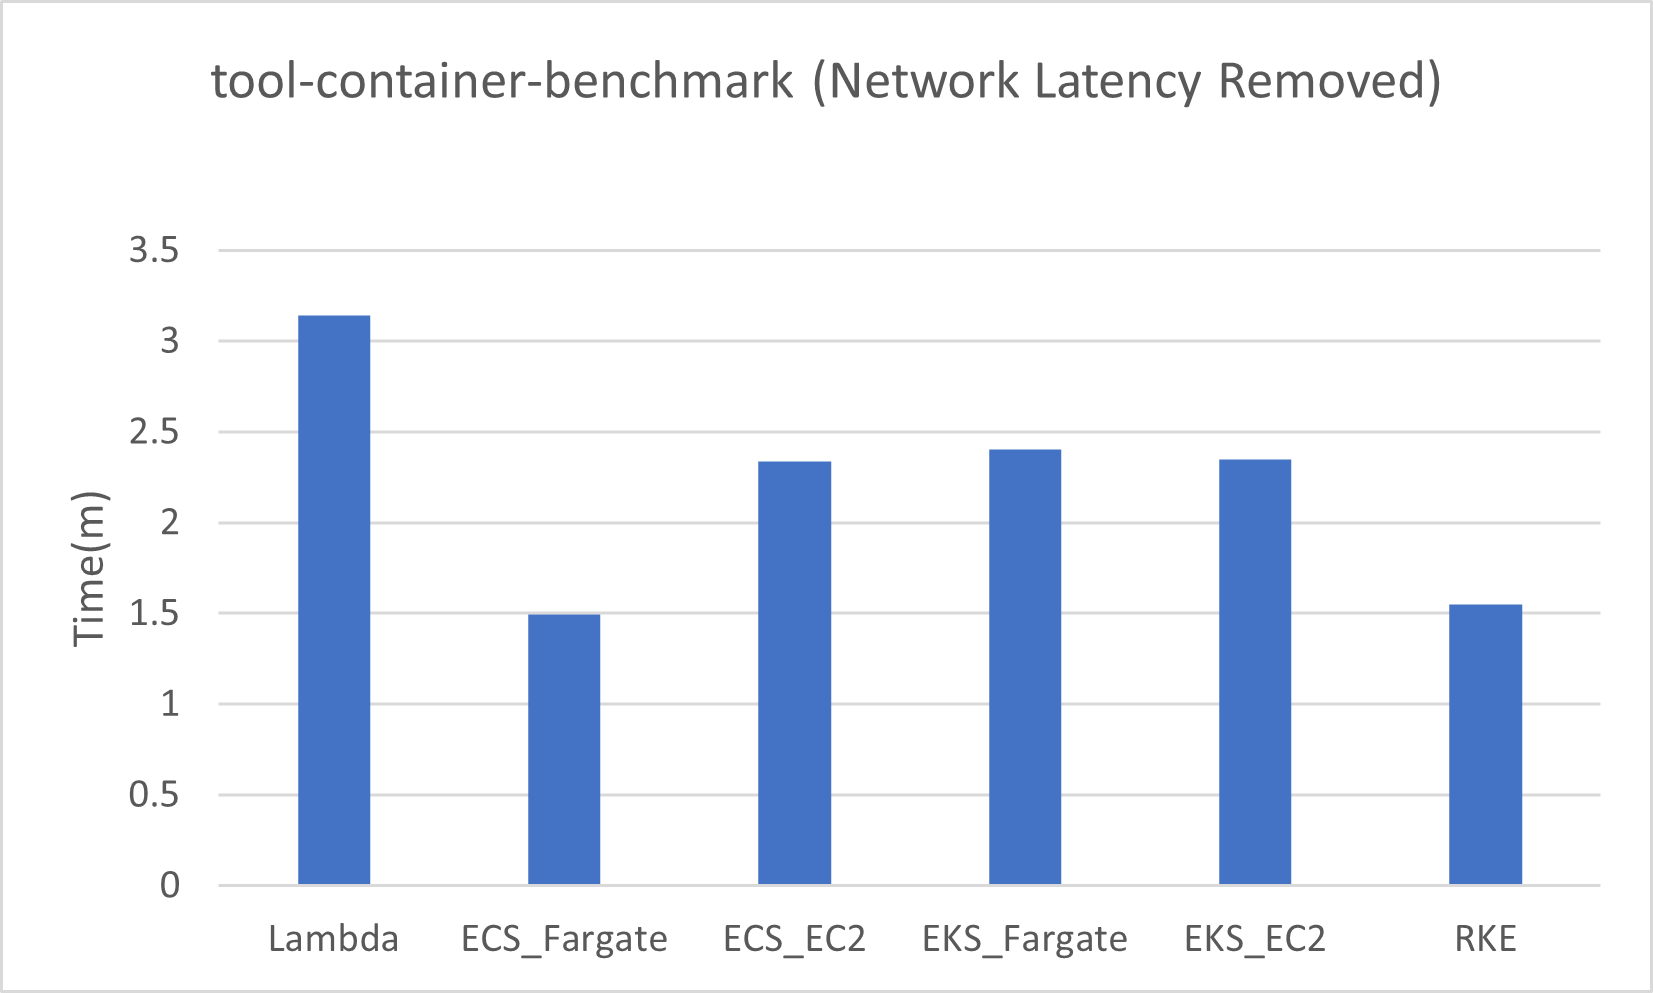
\includegraphics[width=\textwidth]{images/perf-tcb_network.png}
  \caption{\emph{Performance}:Average amount of time required to complete tool-container-benchmark, measured against Database closest to instance 
  (number\_of\_events=30000) --- lower is better}
  \label{fig:perf_tcb_network}
\end{figure}

Even with the extreme network latency caused by the database, a clear performance difference is seen by the \textit{on-premise} series in both Figures\ref{fig:perf_tcb_default} and Figures\ref{fig:perf_tcb_30000}
when comparing between the various instances (excluding the baseline instance).

Figure \ref{fig:perf_tcb_network} compares the results of each instance with the database located closest to it (in an effort to remove network latency as a factor of comparison) with \textit{number-of-events} set to 30000,
which continues to illustrate the pattern of \textit{EKS} performing better than \textit{ECS},
and \textit{EC2} backed instances performing better than their \textit{fargate} backed instances.


\subsection{Cost}
Figure\ref{fig:cost_workload} illustrates the difference in average costing when running \emph{tool-container-benchmark} three times with 30000 events against an \textit{RDS} instance, measured in US Dollars.
This table includes the dollar costing of running the actual workload (for the given period) and the cost of all dependencies,
this may include the environment or required additional services like an \textit{ALB}, over a given period.
The \textit{Serverless} instances have the advantage with \textit{Lambda} costing the lowest amount, followed by the \textit{fargate} backed \textit{ECS} and \textit{EKS} instances.
The two \textit{EC2} instances follow with \textit{ECS} and \textit{EKS} respectively.

Table\ref{fig:cost_projected} projects the costing of running a long-lived services on each platform. Here we see the two \textit{ECS} backed instances taking the lead,
with two \textit{EKS} backed instances following. For both of the above results, when scaling the cost of an \textit{EC2} instance to a cost per container
(as a single \textit{VM} can run 32 containers of the tested spec at the same cost), \textit{fargate} begins to exceed the cost of \textit{EC2}.
Additionally the \textit{EKS} platform cost is per cluster (not per container workload), therefore the additional \$73 cost per month of \textit{EKS} needs to be seen in the context of the amount of workloads being run on a cluster.
It should be noted that due to \textit{Lambda}'s time-limitation of 15 minutes, the value in this table is a theoretical project based on cost per second.

\begin{figure}[htbp]
  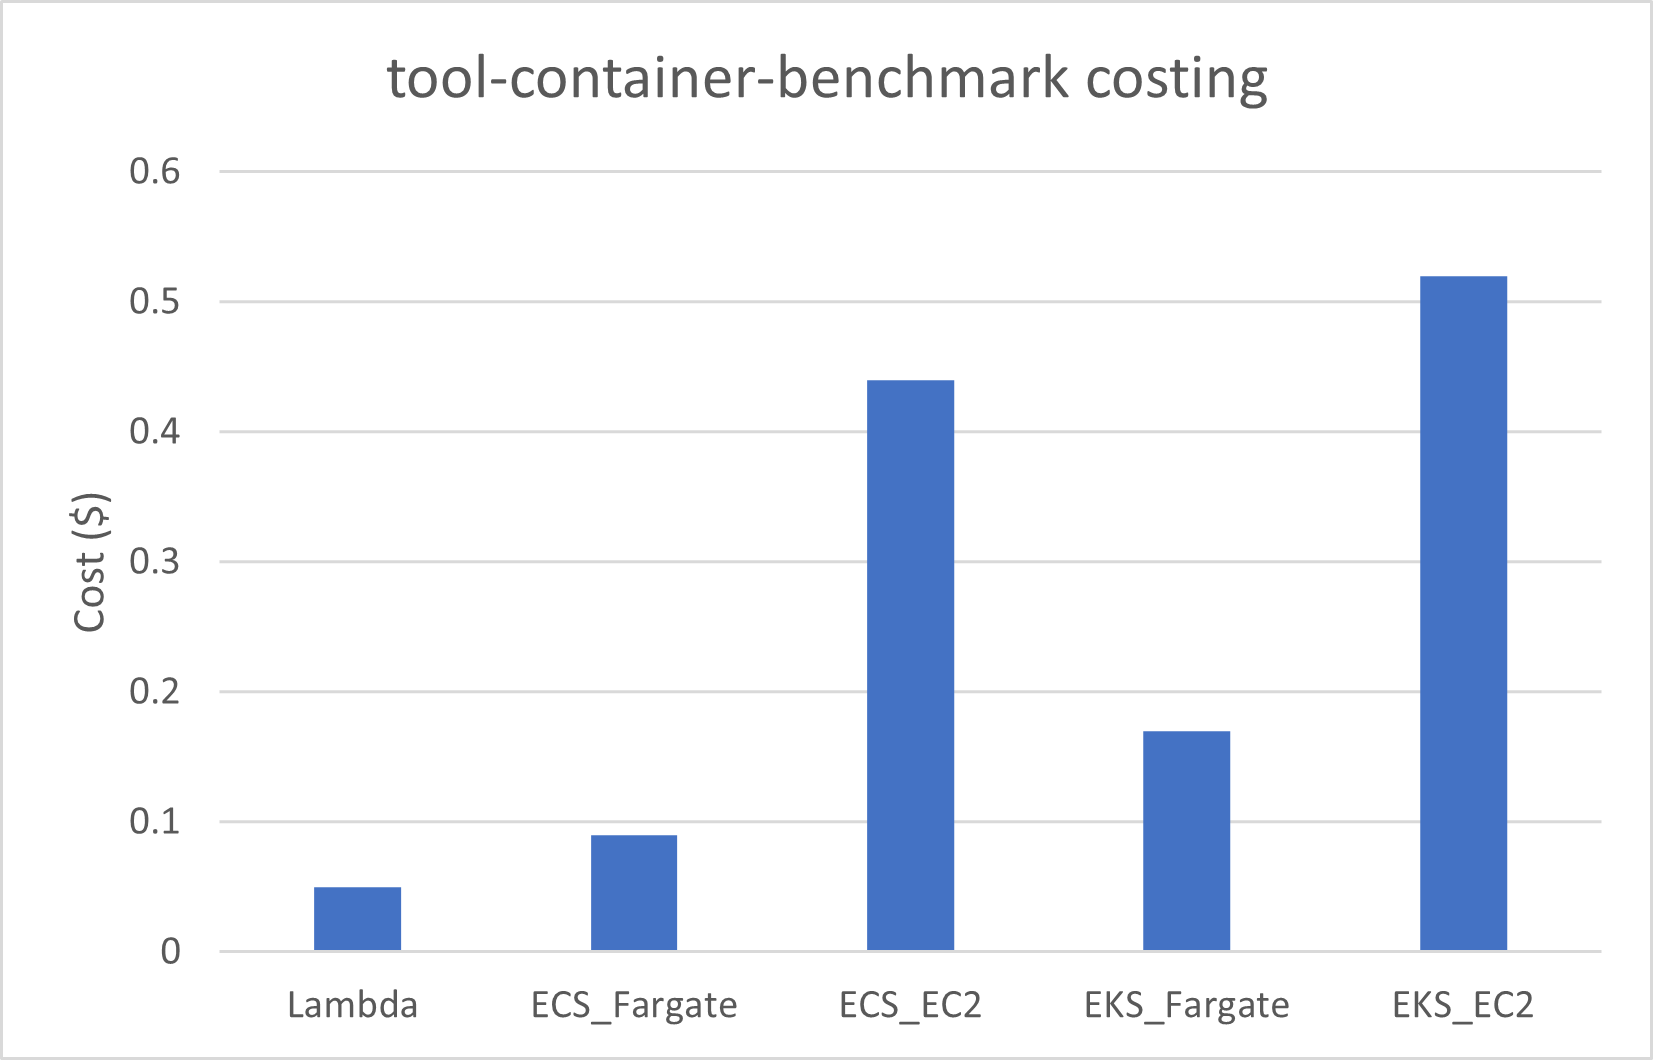
\includegraphics[width=\textwidth]{images/cost-workload.png}
  \caption{\emph{Cost}: Average cost of running \emph{tool-container-benchmark} with 30000 events --- lower is better}
  \label{fig:cost_workload}
\end{figure}

\begin{table}[htbp]
  \caption{\emph{Cost}: Projected costing (\$) of running a sample long-lived service per solution for a month and year}
  \small
  \begin{tabularx}{1\textwidth}{X | X | X }
    \space            & \bf{Monthly} & \bf{Annually} \\
    \hline
    \bf{Lambda      } & 120.11       & 1441.32       \\
    \bf{ECS\_Fargate} & 40.99        & 491.88        \\
    \bf{ECS\_EC2    } & 40.62        & 487.48        \\
    \bf{EKS\_Fargate} & 113.99       & 1367.88       \\
    \bf{EKS\_EC2    } & 113.62       & 1363.48       \\
  \end{tabularx}
  \label{fig:cost_projected}
\end{table}


\subsection{Resilience and Reliability}
Each platform was subjected to \textit{Chaos-Engineering} style tests to assert a level of resilience and reliability under extreme circumstances.

Figure\ref{fig:rr_scaling} illustrates the average amount of \textit{downtime} when scaling down the number of container-workloads to 0 and back to 1, measured in seconds.
The two \textit{EC2} backed workloads completed the scaling in the quickest, with \textit{EKS} completing first, followed by \textit{ECS}.
The two \textit{fargate} workloads followed, with \textit{ECS} completing 33\% quicker than \textit{EKS}.
It should be noted that due to inability to scale \textit{Lamda} functions, it did not participate in this test.

Figure\ref{fig:rr_deleteContainer} illustrates the average amount of time taken between a container workload being forcibly killed, and the workload being restarted, and ready to respond.
\textit{EKS} once again responded to this 35\% quicker than the \textit{ECS} workload, where the controller still noted the removed container as active and ready.
It should be noted that due to the \textit{Serverless} nature of both \textit{Lambda} and \textit{fargate}, neither of these participated in this test.

Figure\ref{fig:rr_reboot} illustrates the average amount of time taken between an underlying host being rebooted unexpectedly, the workload being restarted, and ready to respond.
\textit{ECS} handled the scale-in process 17\% faster than its \textit{EKS} counter-part.
It should be noted that due to the \textit{Serverless} nature of both \textit{Lambda} and \textit{fargate}, neither of these participated in this test.

\begin{figure}[htbp]
  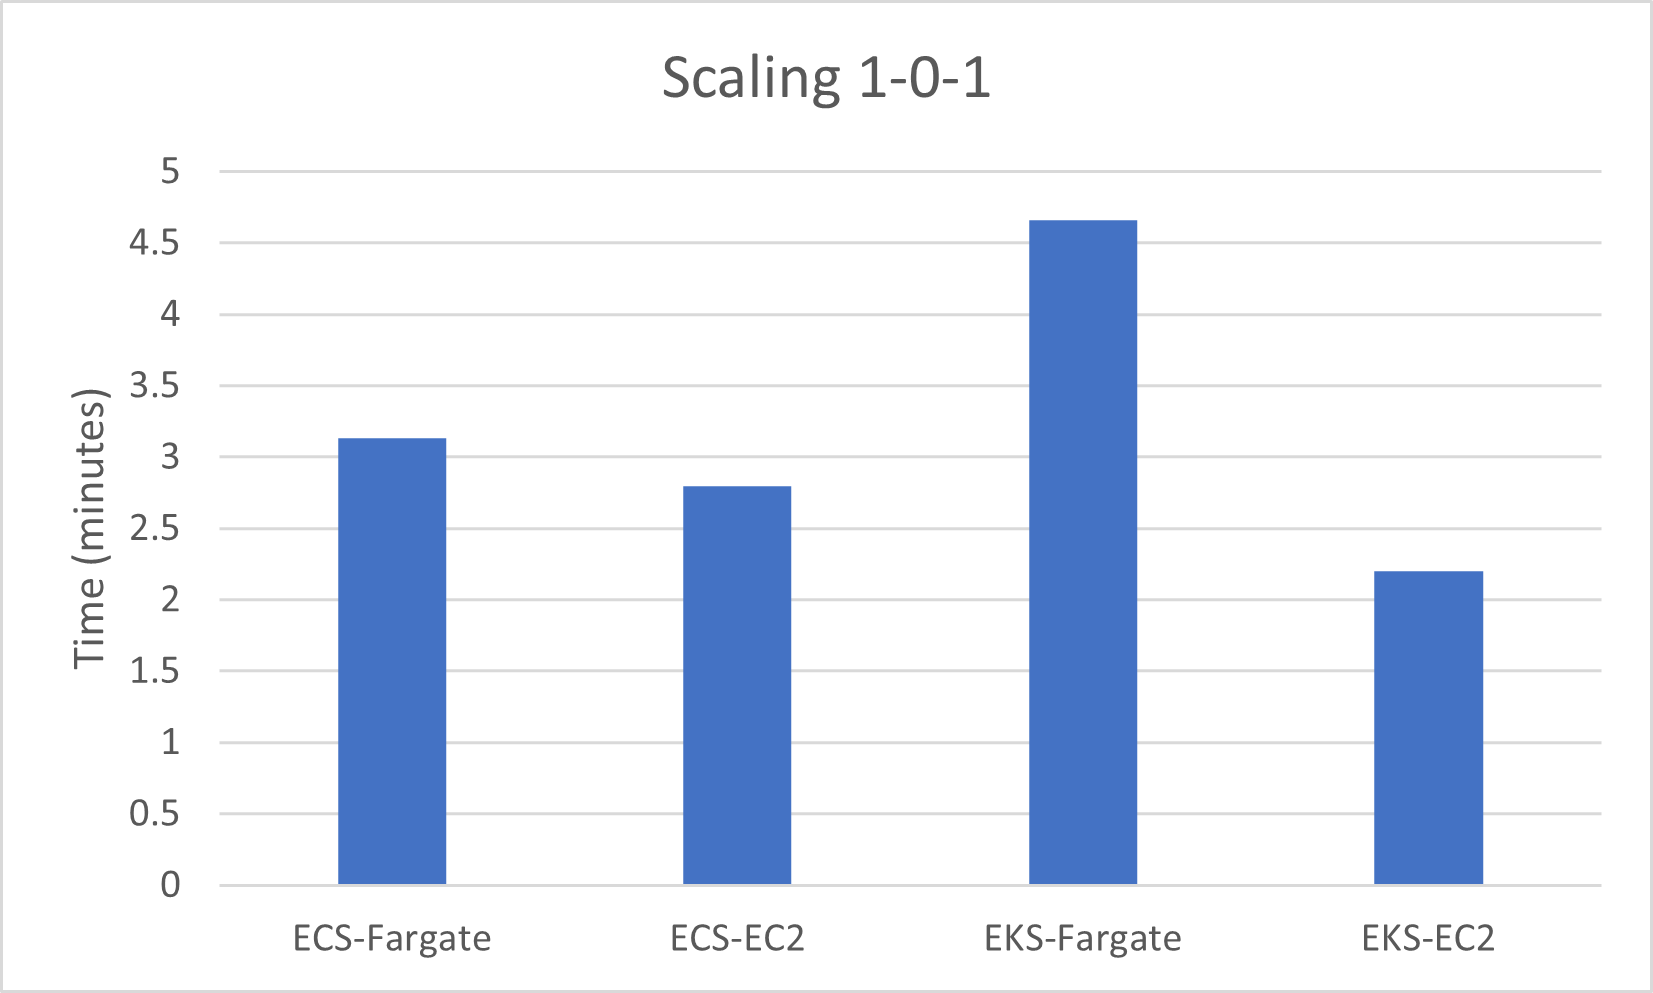
\includegraphics[width=\textwidth]{images/rr-scaling.png}
  \caption{\emph{Resilience and Reliability}: Average amount of downtime measured between scaling operations from one instance, to no instances, and back to one instance --- lower is better}
  \label{fig:rr_scaling}
\end{figure}

\begin{figure}[htbp]
  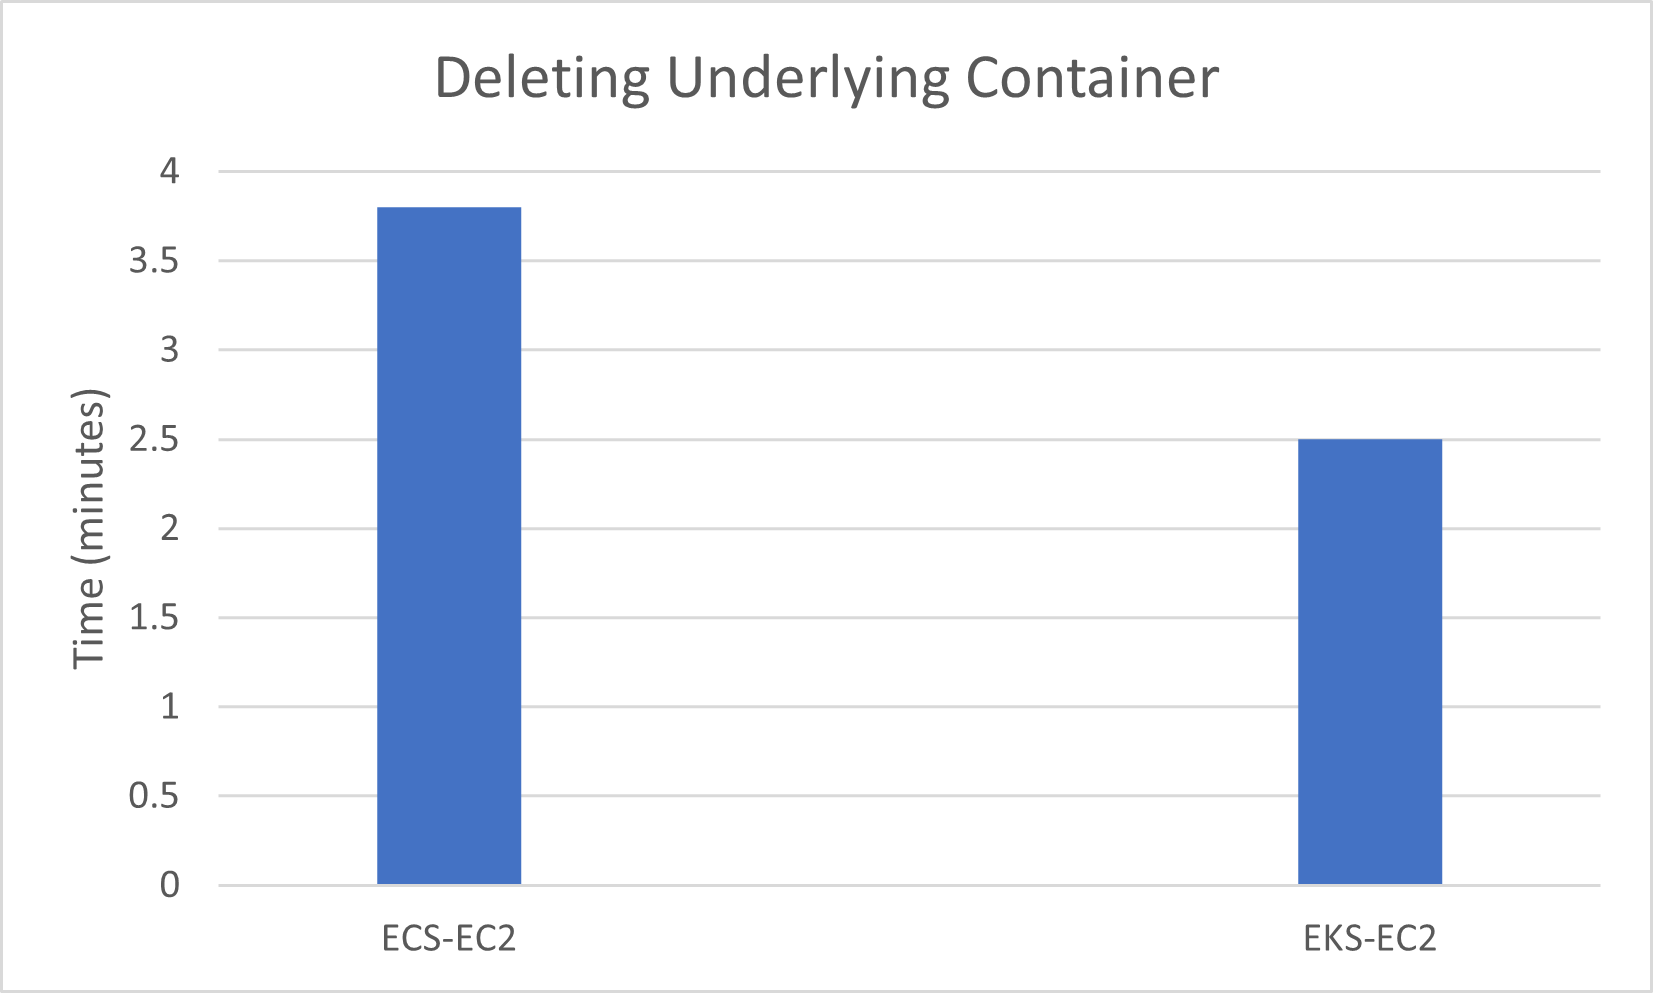
\includegraphics[width=\textwidth]{images/rr-deleteContainer.png}
  \caption{\emph{Resilience and Reliability}: Average amount of downtime measured between deleting a container on underlying host and creation of new container instance --- lower is better}
  \label{fig:rr_deleteContainer}
\end{figure}

\begin{figure}[htbp]
  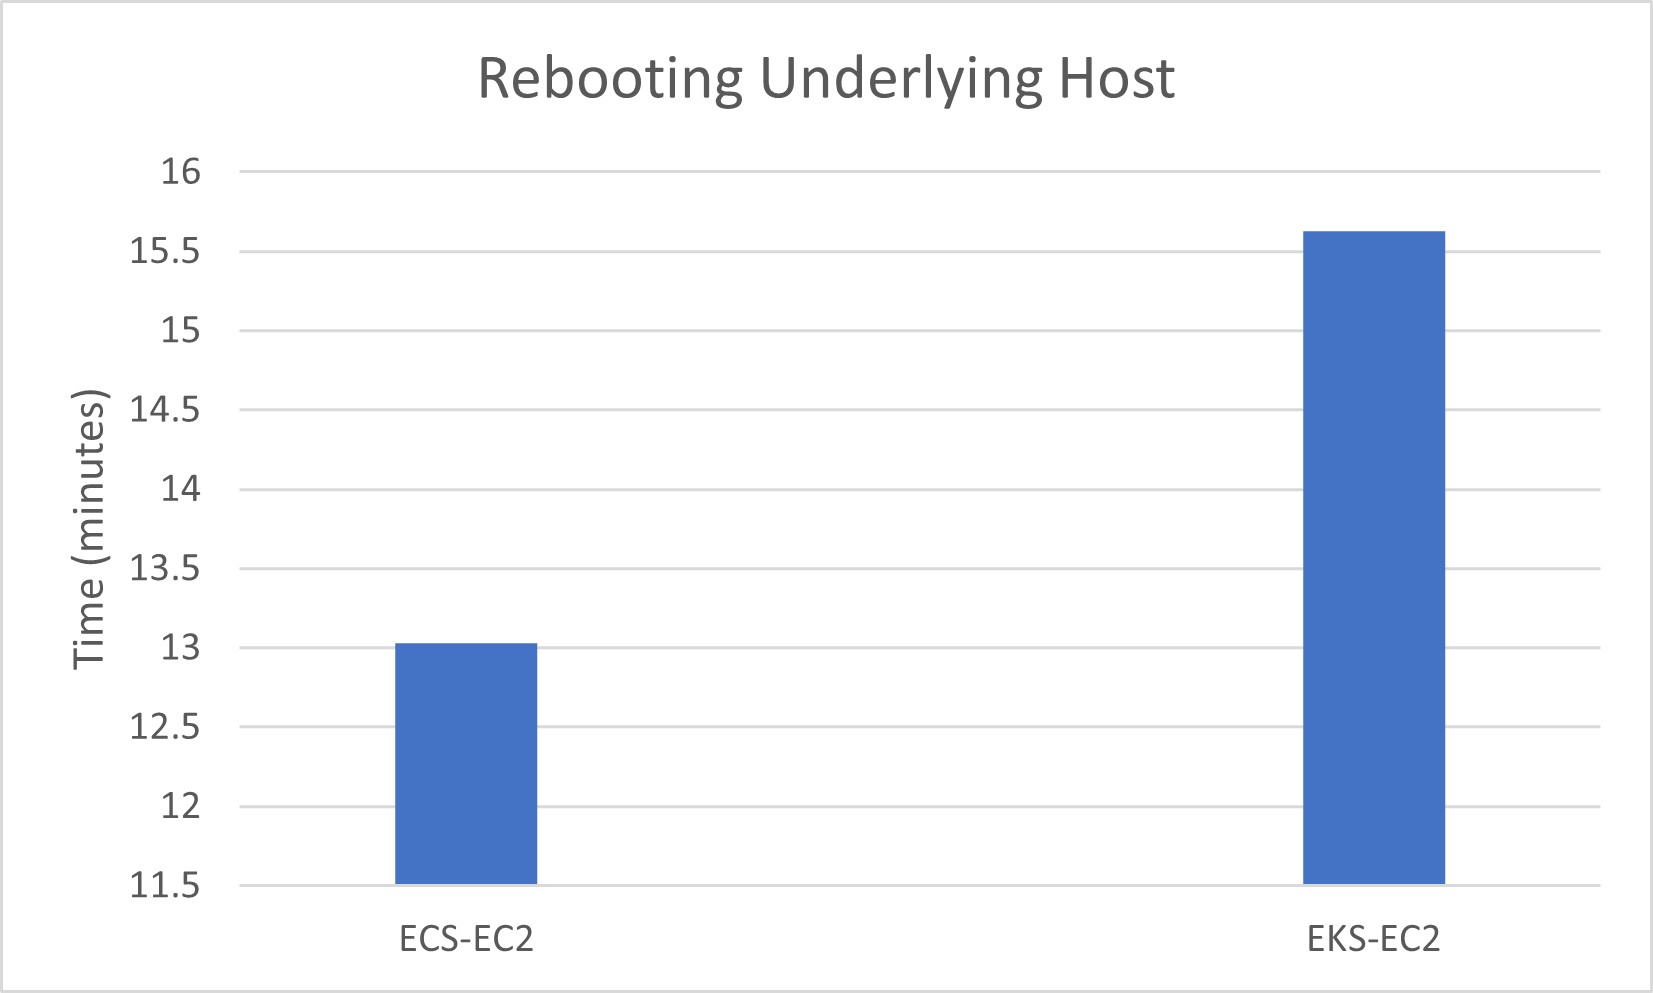
\includegraphics[width=\textwidth]{images/rr-reboot.png}
  \caption{\emph{Resilience and Reliability}: Average amount of downtime measured between deleting a container on underlying host and creation of new container instance --- lower is better}
  \label{fig:rr_reboot}
\end{figure}


\subsection{Ease-of-Use}
Each platform chosen required an architectural design, object configuration, and environment deployment.
In addition, once every environment was ready, a deployment process needed to be designed to run our test workloads on the selected platforms.

\subsubsection{Lambda}
\textit{Lambda} proved to be the easiest environment to get configured, as there was no real environment to create. Being a serverless function,
to run, it required that a Docker image exist (at this moment restricted to \textit{ECR} repositories only with a max image size of 10GB), environment variables to exist and be configured, max amount of memory
and a maximum timeout (being less than 15 minutes). This however, came at an extreme cost of flexibility and configuration.
\textit{Lambdas} being serverless \emph{functions} meant that the expected workload was a function (that is to perform a single task quickly which accepted a specific payload and response),
meant that most of the selected benchmarks were incompatible with the underlying architecture (due to the max size of 10GB of ephemeral storage available).
Where it was possible to run, the code had to be altered significantly and cater for specific \textit{Lambda} requirements.

Deployments of workloads occur via the AWS API (using the CLI, Web-Console or other tools like Terraform)

\subsubsection{ECS}
\textit{ECS} being a cloud-native \textit{orchestration} proved fairly simple to create and configure.
A \emph{cluster} needed to be created (which simply required a unique name), with \textit{capacity-providers} being registered to the cluster,
which can be of type \textit{fargate} or \textit{EC2}.
This process occurs almost immediately, and workloads can be scheduled once a providers is registered.
Workloads are defined using a \textit{task-definition}, a JSON file which describes the intended container-workloads.
Ingress connectivity would be allowed via an external \textit{ALB} which plugs directly into the rest of the architecture.

Running workloads on \textit{fargate}, being \textit{serverless} took little to no effort, as no additional resources needed to be created or configured.
Running workloads on \textit{EC2}, required far more effort, as \textit{AMI}'s needed to be built with the required \textit{ECS} agent (and dependencies) installed, tested,
and configured. Additionally \textit{ASG}'s needed to be configured and registered with the \textit{ECS} cluster before workloads would be scheduled.

Deployments of workloads occur via the AWS API (using the CLI, Web-Console or other tools like Terraform)

\subsubsection{EKS}
A bare \textit{EKS} required a similar amount of effort to create, configure as \textit{ECS}. A \emph{cluster} is created with basic configuration requirements,
further add-ons are then installed separately to add additional features required to get a \textit{k8s} cluster working in the cloud environment.
This process can take up to 30 minutes to complete.
\textit{Worker} instances are then registered to the \textit{EKS} cluster (either \textit{EC2} or \textit{fargate}).
Workloads are defined using using standard \textit{k8s} YAML object files (depending on the object type desired).
For users unfamiliar with the \textit{k8s} architecture, this can be a source of great complexity and new tooling requirements.
Ingress connectivity requires an additional ingress-controller component to be deployed into the cluster, coupled with an \textit{ALB}.

Running workloads on \textit{fargate} and \textit{EC2} is quite similar in complexity to \textit{ECS}.

Deployments of workloads occur via a specific AWS tool called \emph{eksctl}\cite{weaveworks} or the standard \textit{k8s} deployment tool \emph{kubectl}\cite{kubectl}

Figure\ref{fig:eou} illustrates the amount of time taken to bootstrap and configure each platform to be ready to run workloads (measured in minutes).
and the amount of time required to convert an existing container workload to run on each platform (measured in minutes).

\begin{figure}[htbp]
  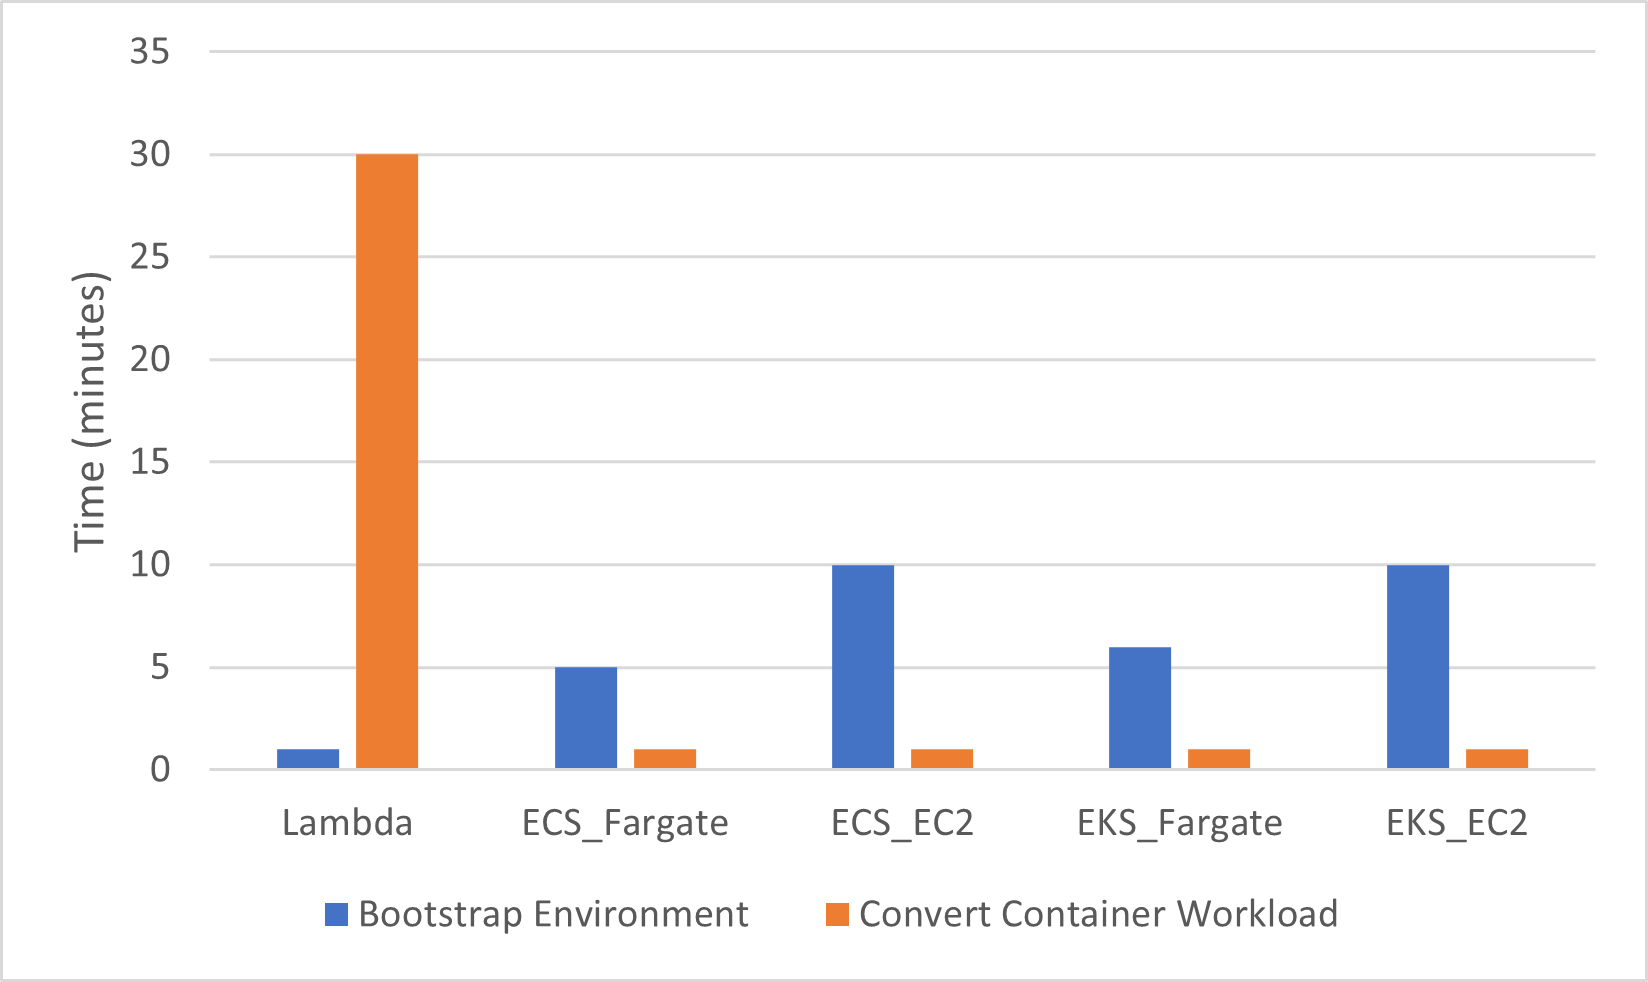
\includegraphics[width=\textwidth]{images/eou.png}
  \caption{\emph{Ease-of-Use}: Amount of time taken to complete environmental bootstrap and convert an existing container workload to run on solution --- lower is better}
  \label{fig:eou}
\end{figure}

\part{Discussion and Conclusion}

This chapter evaluates the aforementioned results in context of the posed problem.
Additionally a concluding solution is presented, with potential future-work mentioned.

\chapter{Discussion}

\section{Performance and Latency}
\section{Ease-of-Use}

\section{Cost}

\section{Resilience and Reliability}

\chapter{Conclusion}
Based on the experimentation results presented and aforementioned argued points, the following conclusions are be made
\begin{itemize}
  \item selection of container-orchestration solution will have a minor impact on performance for certain workloads
        \begin{itemize}
          \item \textit{EKS} running workloads generally performed closer to the benchmark cluster across the widest array of tests,
                with both \textit{ECS}, followed by \textit{Lambda}, lagging constantly behind, with low, but measurable performance impact.
        \end{itemize}
  \item selection of underlying server-architecture has a far more significant impact on performance for most workloads
        \begin{itemize}
          \item \textit{EC2} based workloads consistently performed closer (or on occasion out-performed) our benchmark cluster,
                whilst both \textit{Serverless} options (\textit{Fargate} and \textit{Lambda} respectively) producing lower performance,
                even under the same orchestration solution
        \end{itemize}
  \item Network latency does not mask the loss in (measurable) performance between the various orchestration solutions or underlying server-architecture
        \begin{itemize}
          \item Benchmarks showed a consistent degradation in performance between the tested solutions, irrespective of network latency.
        \end{itemize}
  \item Whilst \textit{Serverless Functions} may have the ability to run container-based workloads,
        the numerous limitations of attempting to run standard container-workloads on a
        \textit{Serverless} architectural design, makes it an inviable replacement for an existing container-orchestration solution
  \item \textit{Cloud-Native} container orchestration solutions generally offer a more \emph{consistent} experience
        (in context to the rest of the chosen \textit{cloud} provider's environment), with simpler tie-ins to other offered services, and marginally lower costs.
        These \emph{ease-of-use} factors are off-set by a measurable loss in performance, marginal (yet observable) lower level of resiliency, provider \textit{lock-in},
        and limited support.
  \item Managed Cloud \textit{Kubernetes} solutions benefit from utilizing an \textit{open-sourced}, \emph{ubiquitos} and near \textit{standard} solution
        that a \textit{k8s} cluster offers (this include that existing tooling would require little-to-no changes as part of the migration process),
        at the cost of complexity (in terms of tie-ins to other cloud offered services) and monthly costing.
\end{itemize}

\chapter{Future Work}


\backmatter
% References
% No restriction is set to the reference styles
% Save your references in References.bib
\nocite{*} % Remove this for your own citations
\bibliographystyle{IEEEtran}
\bibliography{References}

\appendix
\chapter{Docker Image Definitions}
\label{appendix:docker_images}

\section{tool-benchmarking-suite}

\begin{minted}[tabsize=2,breaklines]{bash}
FROM ubuntu:20.04

ENV DEBIAN_FRONTEND=noninteractive \
  TZ=Africa/Johannesburg

# Sysbench
RUN  apt-get -y install curl && \
  curl https://packagecloud.io/install/repositories/akopytov/sysbench/script.deb.sh | bash && \
  apt -y install sysbench

# Phoronix 
RUN apt-get -y install php-cli php-common php-xml && \ 
  wget https://phoronix-test-suite.com/releases/repo/pts.debian/files/phoronix-test-suite_10.8.2_all.deb && \
  dpkg -i phoronix-test-suite_10.8.2_all.deb
RUN apt-get install -y build-essential zlib1g-dev 

# Phoronix tests
RUN phoronix-test-suite batch-install \
  pts/compress-7zip-1.8.0 \
  pts/mbw-1.0.0 \ 
  pts/ramspeed-1.4.3 \ 
  pts/fs-mark-1.0.3 \ 
  pts/redis-1.3.1 \ 
  pts/m-queens-1.1.0 
COPY phoronix-test-suite.xml /etc/
COPY suite-definition.xml /var/lib/phoronix-test-suite/test-suites/local/containerbenchmark/

# AWS CLI
RUN curl "https://awscli.amazonaws.com/awscli-exe-linux-x86_64.zip" -o "awscliv2.zip" && \
  unzip awscliv2.zip && \
  ./aws/install && \
  rm -rf "awscliv2.zip"

RUN apt -y install python3

COPY scripts/run.sh /root/

CMD ["/root/run.sh"]
\end{minted}

\section{tool-container-benchmark}
\begin{minted}[tabsize=2,breaklines]{bash}
  FROM golang
  ONBUILD COPY ./src/service /service
  CMD ["/service"]
\end{minted}
\chapter{packer AMI Definitions}
\label{appendix:packer_ami_defintions}

\section{ECS}
\subsection*{ami.pkr.hcl}
\begin{minted}[tabsize=2,breaklines]{bash}
  packer {
    required_plugins {
      amazon = {
        version = ">= 0.0.1"
        source  = "github.com/hashicorp/amazon"
      }
    }
  }
  
  source "amazon-ebs" "ag-ret-ecs" {
    ami_description = "An AMI that has required ECS components"
    ami_name      = "ag-ret-ecs-{{timestamp}}"
    instance_type = "t3.micro"
    region         = var.region
  
    ssh_username   = "ubuntu"
  
    launch_block_device_mappings {
      device_name           = "/dev/sda1"
      encrypted             = true
      delete_on_termination = true
      volume_size           = 100
      volume_type           = "gp2"
    }
    
    subnet_filter {
      filters = {
        "tag:tier" = "compute"
      }
      most_free = true
      random    = true
    }
    
    vpc_filter {
      filters = {
        "tag:Name": "ag-ret-${var.environment}-${var.region}",
      }
    }
  
    source_ami_filter {
      filters = {
        name                = "lib-ami-ubuntu-retail*"
        root-device-type    = "ebs"
        virtualization-type = "hvm"
      }
      owners      = ["860638170744"] # global-shared
      most_recent = true
    }
    
    tags = local.tags
    run_tags = local.tags
    run_volume_tags = local.tags
  }
  
  build {
    sources = ["source.amazon-ebs.ag-ret-ecs"]
    provisioner "shell" {
      script          = "provision.sh"
      execute_command = "{{.Vars}} sudo -E bash '{{.Path}}'"
    }
    post-processor "manifest" {
      output     = "manifest.json"
      strip_path = true
    }
  }  
\end{minted}

\subsection*{provision.sh}
\begin{minted}[tabsize=2,breaklines]{bash}
#!/bin/bash
# https://github.com/aws/amazon-ecs-agent
set -eo pipefail

export DEBIAN_FRONTEND=noninteractive 

cloud-init status --wait

# Install Docker
set +e
apt remove docker docker-engine docker.io containerd runc
set -e
apt update
apt install -y \
    ca-certificates \
    curl \
    gnupg \
    lsb-release
curl -fsSL https://download.docker.com/linux/ubuntu/gpg | apt-key add -
add-apt-repository "deb [arch=amd64] https://download.docker.com/linux/ubuntu $(lsb_release -cs) stable"
apt update && apt install -y docker-ce docker-ce-cli containerd.io
usermod -aG docker ubuntu
systemctl enable docker

# Create ECS folders 
mkdir -p /var/log/ecs /etc/ecs /var/lib/ecs/data
touch /etc/ecs/ecs.config

# Set up necessary rules to enable IAM roles for tasks
sysctl -w net.ipv4.conf.all.route_localnet=1
iptables -t nat -A PREROUTING -p tcp -d 169.254.170.2 --dport 80 -j DNAT --to-destination 127.0.0.1:51679
iptables -t nat -A OUTPUT -d 169.254.170.2 -p tcp -m tcp --dport 80 -j REDIRECT --to-ports 51679
\end{minted}

\section{EKS}
\subsection*{ami.pkr.hcl}
\begin{minted}[tabsize=2,breaklines]{bash}
packer {
  required_plugins {
    amazon = {
      version = ">= 0.0.1"
      source  = "github.com/hashicorp/amazon"
    }
  }
}

source "amazon-ebs" "ag-ret-eks" {
  ami_description = "An AMI that has required eks components"
  ami_name      = "ag-ret-eks-{{timestamp}}"
  instance_type = "t3.micro"
  region         = var.region

  ssh_username   = "ubuntu"

  launch_block_device_mappings {
    device_name           = "/dev/sda1"
    encrypted             = true
    delete_on_termination = true
    volume_size           = 100
    volume_type           = "gp2"
  }
  
  subnet_filter {
    filters = {
      "tag:tier" = "compute"
    }
    most_free = true
    random    = true
  }
  
  vpc_filter {
    filters = {
      "tag:Name": "ag-ret-${var.environment}-${var.region}",
    }
  }

  source_ami_filter {
    filters = {
      name                = "ubuntu-eks/k8s_1.20/images/
        hvm-ssd/ubuntu-focal-20.04-amd64-server-2022*"
      root-device-type    = "ebs"
      virtualization-type = "hvm"
    }
    owners      = ["099720109477"] # canonical
    most_recent = true
  }
  
  tags = local.tags
  run_tags = local.tags
  run_volume_tags = local.tags
}

build {
  sources = ["source.amazon-ebs.ag-ret-eks"]

  provisioner "file" {
    source      = "sources.list"
    destination = "/tmp/sources.list"
  }
  provisioner "shell" {
    script          = "provision.sh"
    execute_command = "{{.Vars}} bash '{{.Path}}'"
  }
  post-processor "manifest" {
    output     = "manifest.json"
    strip_path = true
  }
}

\end{minted}

\subsection*{provision.sh}
\begin{minted}[tabsize=2,breaklines]{bash}
#!/bin/sh
set -e

sudo apt-get -y install awscli

sudo apt-get -y autoremove
sudo apt-get -y clean
\end{minted}

\end{document}